\documentclass[10pt]{article}
\usepackage[utf8]{inputenc}
\usepackage[italian]{babel}
\usepackage{graphicx} 
\usepackage{amsmath}
\usepackage{float}
\usepackage{listings}
\usepackage{xcolor} 
\usepackage{hyperref} 

\begin{document}

\begin{titlepage}
    \centering
    % Assicurati che il file esista nella cartella del progetto con questo nome esatto
    
\includegraphics[width=0.45\textwidth]{img/logo_unipr.png} \\[0.5cm]

    {\large \textbf{DIPARTIMENTO DI INGEGNERIA E ARCHITETTURA}} \\[0.2cm]
    {\normalsize CORSO DI LAUREA IN INGEGNERIA INFORMATICA, ELETTRONICA E DELLE TELECOMUNICAZIONI} \\[2.5cm]

    {\Large \textbf{Adattamento e valutazione di Tiny Recursive Model per il gioco de Go}} \\[2cm]

    \begin{minipage}[t]{0.48\textwidth}
        \begin{flushleft}
            \textbf{Relatore:} \\
            Prof. Michele Tomaiuolo \\[0.4cm]
        \end{flushleft}
    \end{minipage}
    \hfill
    \begin{minipage}[t]{0.48\textwidth}
        \begin{flushright}
            \textbf{Laureando:} \\
            Francesco Maria Vescovi
        \end{flushright}
    \end{minipage}

    \vfill

    {\normalsize \textbf{ANNO ACCADEMICO 2025 -- 2026}}
\end{titlepage}

\tableofcontents
\clearpage

\section{Introduzione}

\subsection{Contesto}

Il gioco del Go rappresenta un interessante ambito di applicazione per lo studio e lo sviluppo di sistemi di intelligenza artificiale.

Nonostante la semplicità delle sue regole, il gioco presenta una complessità strategica particolarmente elevata, dovuta all'ampiezza dello spazio delle possibili configurazioni e alla difficoltà di valutare le conseguenze delle singole mosse.

Queste caratteristiche rendono il Go un interessante banco di prova per lo sviluppo di sistemi basati su tecniche di apprendimento automatico e reti neurali.

Un ulteriore elemento che contribuisce alla complessità del gioco è rappresentato dalla sua natura dinamica e competitiva. A ogni turno, infatti, il giocatore deve selezionare una mossa tenendo conto non soltanto della configurazione corrente della scacchiera, ma anche delle possibili risposte dell'avversario e delle conseguenze che queste possono produrre nelle fasi successive della partita.

Il numero di azioni disponibili è inoltre particolarmente elevato: su una scacchiera standard di dimensioni 19×19 sono presenti 361 possibili intersezioni nelle quali collocare una pietra, a cui si aggiunge la possibilità di passare il turno. Questo comporta uno spazio di ricerca molto ampio, rendendo particolarmente complessa la valutazione delle mosse e delle relative conseguenze.

Negli ultimi anni, l'evoluzione dei metodi di apprendimento automatico ha permesso di realizzare agenti sempre più sofisticati, capaci di apprendere strategie di gioco a partire dai dati e di selezionare le mosse più efficaci.

Un risultato particolarmente significativo in questo ambito è stato raggiunto nel marzo 2016, quando AlphaGo, un algoritmo sviluppato da Google DeepMind che combinava apprendimento supervisionato (supervised learning) e apprendimento per rinforzo (reinforcement learning), ha ottenuto un risultato fino ad allora ritenuto impossibile, sconfiggendo il campione mondiale Lee Sedol \cite{alphago}.

I risultati ottenuti da sistemi specializzati dimostrano le potenzialità delle tecniche di apprendimento automatico applicate al gioco del Go. Tuttavia, l'impiego di modelli progettati specificamente per un determinato dominio pone una questione differente rispetto all'utilizzo di architetture più generali.

In quest'ultimo caso, l'interesse non risiede esclusivamente nella capacità di risolvere il problema considerato, ma anche nella possibilità di riutilizzare una struttura esistente, adattandone le componenti necessarie per affrontare compiti differenti.

Questo approccio permette di indagare la flessibilità dell'architettura e i suoi limiti al di fuori del contesto per il quale è stata originariamente concepita.

\subsection{Obiettivo della tesi}

Tiny Recursive Model (TRM) \cite{trm} è un modello di rete neurale caratterizzato da un'architettura ricorsiva basata su transformer, progettato per risolvere problemi deterministici, statici e a singolo agente, quali sudoku e labirinti. La sua architettura si basa sull'utilizzo di un numero contenuto di parametri e sull'applicazione iterativa dei medesimi blocchi di rete, consentendo di elaborare progressivamente le informazioni e affinare le predizioni.

L'obiettivo della tesi è adattare Tiny Recursive Model al gioco del Go, verificando la capacità dell'architettura di affrontare una tipologia di problema sostanzialmente diversa da quelle per cui è stata originariamente progettata. Si tratta, infatti, di un problema anch'esso deterministico, ma caratterizzato da una complessità computazionale significativamente maggiore, nonché da un ambiente variabile e multi-agente.

L'adattamento ha richiesto interventi su diverse componenti del modello, mantenendo come elemento centrale, e per quanto possibile intatto, la struttura ricorsiva originale. In particolare, è stato necessario modificare la rappresentazione dello stato del gioco, affinché il modello potesse elaborare la configurazione della scacchiera, e introdurre una componente di output specifica per la previsione delle mosse, attraverso la quale vengono assegnate probabilità alle possibili azioni.

È stata inoltre sviluppata la logica necessaria per interpretare le predizioni del modello e selezionare una mossa valida, tenendo conto delle regole del gioco. Il processo di apprendimento è stato invece basato sull'utilizzo di partite registrate in formato SGF, dalle quali ricavare gli esempi necessari all'addestramento.

Oltre alla realizzazione dell'implementazione, il lavoro prevede una fase di valutazione sperimentale volta ad analizzare il comportamento del modello nelle diverse configurazioni considerate.

In particolare, vengono prese in esame due dimensioni della scacchiera, 9×9 e 19×19, al fine di valutare le prestazioni del modello in contesti caratterizzati da differenti livelli di complessità. Viene inoltre analizzato l'impatto dell'utilizzo dell'algoritmo Negamax, impiegato come componente strategica a supporto del processo di selezione delle mosse, confrontando le configurazioni che ne prevedono l'impiego con quelle che non lo utilizzano.

Infine, le prestazioni dell'agente vengono valutate attraverso confronti con KataGo, un motore di gioco per il Go utilizzato come riferimento nella fase sperimentale. Tale confronto permette di ottenere un'indicazione del livello di gioco raggiunto dal modello e di analizzare i limiti dell'approccio adottato.

\subsection{Struttura della tesi}

La tesi è organizzata in sei capitoli, ciascuno dedicato a uno specifico aspetto del progetto.

Il primo capitolo introduce il problema affrontato, ne descrive il contesto e presenta gli obiettivi del lavoro.

Il secondo capitolo è dedicato al background teorico e tecnologico. Vengono approfonditi lo stato dell'arte, le tecnologie utilizzate e i componenti preesistenti sui quali si basa il progetto, fornendo le conoscenze necessarie alla comprensione delle modifiche successivamente introdotte.

Il terzo capitolo descrive l'architettura del sistema sviluppato, illustrandone le principali componenti, le modifiche apportate rispetto alla struttura originale e le motivazioni alla base delle scelte progettuali.

Il quarto capitolo approfondisce gli aspetti implementativi, analizzando le soluzioni adottate a livello di codice e le principali scelte tecniche che hanno caratterizzato lo sviluppo del sistema.

Il quinto capitolo è dedicato alla valutazione sperimentale. Vengono presentate le metriche utilizzate, le modalità di confronto tra le diverse configurazioni implementate e i risultati ottenuti.

Infine, il sesto capitolo presenta le conclusioni del lavoro, evidenziando i risultati raggiunti, i principali limiti riscontrati e alcuni possibili sviluppi futuri.

\clearpage
\newpage
\section{Background}

\subsection{Il gioco del Go}

Il Go è un gioco da tavolo strategico per due giocatori, originario della Cina e successivamente diffusosi in altri paesi dell'Asia orientale, in particolare in Giappone e Corea. I due giocatori, uno con le pietre nere e l'altro con quelle bianche, si alternano nel posizionamento delle proprie pietre su una scacchiera, con l'obiettivo di conquistare il controllo di una porzione di territorio maggiore rispetto all'avversario.

Il gioco si svolge su una griglia, denominata "goban", costituita da linee orizzontali e verticali che si intersecano formando dei punti di gioco. Le dimensioni tradizionali della scacchiera sono 19×19, per un totale di 361 intersezioni. Sono tuttavia utilizzate anche dimensioni ridotte, come 9×9 e 13×13, particolarmente adatte a partite più brevi e a contesti di apprendimento.

A differenza di altri giochi da tavolo, le pietre non vengono posizionate all'interno delle caselle, ma sulle intersezioni della griglia. Una volta collocata, una pietra rimane nella propria posizione fino a quando non viene eventualmente catturata dall'avversario. Le pietre dello stesso colore che si trovano su intersezioni adiacenti orizzontalmente o verticalmente formano un gruppo e condividono le proprie libertà.

Le libertà rappresentano le intersezioni libere direttamente adiacenti a una pietra o a un gruppo di pietre. Quando un gruppo perde tutte le proprie libertà, viene catturato e rimosso dalla scacchiera. Per questo motivo, durante una partita, i giocatori devono bilanciare l'espansione del proprio territorio con la necessità di proteggere i propri gruppi e limitare le possibilità dell'avversario.

Una regola fondamentale del Go è il divieto di ripetizione immediata della posizione precedente, noto come regola del "ko". Questa impedisce che una sequenza di catture possa generare una ripetizione infinita delle stesse configurazioni. A seconda del regolamento adottato, possono essere previste ulteriori restrizioni sulla ripetizione delle posizioni.

Durante il proprio turno, un giocatore può anche decidere di passare, rinunciando a effettuare una mossa. La partita termina quando entrambi i giocatori passano consecutivamente. Si procede quindi alla determinazione del punteggio, che dipende dal territorio controllato e, in funzione del regolamento adottato, dal numero di pietre catturate e da altri elementi. Vince il giocatore che ottiene il punteggio maggiore.

\subsubsection{Dimensioni della scacchiera}

Sebbene le regole rimangano invariate, le dimensioni della scacchiera influenzano significativamente lo svolgimento della partita e la complessità delle decisioni.

La configurazione 9×9 dispone di 81 intersezioni, un numero sensibilmente inferiore rispetto alle 361 della configurazione 19×19. La riduzione dello spazio di gioco comporta generalmente partite più brevi e una maggiore concentrazione degli scontri in aree ristrette della scacchiera. Questo rende il 9×9 particolarmente adatto a sperimentazioni iniziali e allo studio delle dinamiche fondamentali del gioco.

La scacchiera 19×19, invece, offre uno spazio strategico molto più ampio. Le decisioni non riguardano soltanto gli scontri locali e la sopravvivenza dei singoli gruppi, ma anche il controllo di vaste porzioni di territorio e il rapporto tra le diverse aree della scacchiera. Le mosse possono produrre conseguenze a lungo termine e richiedere una valutazione complessiva della posizione, aumentando sensibilmente la difficoltà del processo decisionale.

\subsubsection{Complessità strategica e scelta delle mosse}

La complessità del Go non deriva esclusivamente dal numero di intersezioni disponibili, ma soprattutto dalle interazioni tra le pietre e dalle conseguenze strategiche delle singole mosse.

A ogni turno, il giocatore deve scegliere tra un insieme di azioni legali, valutando non soltanto gli effetti immediati della propria mossa, ma anche le possibili risposte dell'avversario. Una scelta apparentemente vantaggiosa nel breve periodo può infatti compromettere la posizione complessiva nelle fasi successive della partita.

Inoltre, a differenza di problemi nei quali è possibile determinare una soluzione attraverso una sequenza di operazioni indipendenti dalle decisioni di un avversario, nel Go ogni azione modifica lo stato della scacchiera e influenza le possibilità di entrambi i giocatori.
La valutazione di una mossa deve quindi tenere conto di un ambiente in continua evoluzione e di un processo decisionale competitivo.

Queste caratteristiche rendono particolarmente complessa la ricerca di una strategia efficace. Il numero elevato di mosse possibili, combinato con la profondità delle sequenze di gioco e con la necessità di prevedere le risposte dell'avversario, rende difficile esplorare esaustivamente tutte le possibili evoluzioni della partita. La scelta di una mossa richiede pertanto un processo di valutazione capace di individuare le azioni più promettenti senza dover necessariamente analizzare ogni possibile continuazione.

\subsection{Fondamenti delle reti neurali}

Le reti neurali artificiali (Artificial Neural Networks, ANN) sono modelli computazionali ispirati, in maniera semplificata, al funzionamento delle reti di neuroni biologici. Appartengono alla famiglia dei modelli di apprendimento automatico (machine learning) e permettono di apprendere relazioni e schemi presenti nei dati, al fine di effettuare previsioni o classificazioni.

Una rete neurale è costituita da un insieme di unità computazionali, chiamate neuroni artificiali, organizzate in livelli (layer) e collegate tra loro attraverso connessioni caratterizzate da parametri numerici, denominati pesi (weights). L'elaborazione delle informazioni avviene attraverso la propagazione dei dati da un livello al successivo, trasformando progressivamente la rappresentazione dell'input.

\paragraph{Neuroni e struttura della rete}

Il neurone artificiale rappresenta l'unità fondamentale di una rete neurale. Ogni neurone riceve uno o più valori in ingresso, a ciascuno dei quali viene associato un peso, e calcola una combinazione lineare degli stessi, a cui viene generalmente aggiunto un termine indipendente chiamato bias.

Il risultato viene successivamente elaborato attraverso una funzione di attivazione, che introduce una trasformazione non lineare e determina il valore restituito dal neurone.

In forma semplificata, il funzionamento di un neurone può essere rappresentato dalla seguente espressione:

\[
    y = f\left(\sum_{i=1}^{n} w_i x_i + b\right)
\]

dove \(x_i\) rappresenta ciascun valore in ingresso, \(w_i\) il relativo peso, \(b\) il bias e \(f\) la funzione di attivazione. Il valore \(y\) costituisce l'uscita del neurone.

I neuroni vengono organizzati in livelli con funzioni differenti. Generalmente si distinguono:

\begin{itemize}
    \item \textbf{Input layer:} riceve i dati in ingresso e li rende disponibili alla rete.
    \item \textbf{Hidden layers:} elaborano le informazioni attraverso le trasformazioni effettuate dai neuroni e dalle relative connessioni.
    \item \textbf{Output layer:} produce il risultato finale della rete, che può rappresentare una classificazione, una previsione o un altro tipo di informazione.
\end{itemize}

Il numero di livelli e di neuroni, insieme alla modalità con cui sono collegati, contribuisce a definire l'architettura della rete. Le funzioni di attivazione, invece, permettono di introdurre non linearità nel processo di elaborazione. Tra le più utilizzate si trovano ReLU (Rectified Linear Unit), sigmoid e tanh.

\paragraph{Forward propagation e backpropagation}

L'elaborazione dei dati all'interno di una rete neurale avviene attraverso un processo denominato forward propagation. Durante questa fase, i dati vengono forniti al livello di ingresso e propagati attraverso i livelli successivi, fino a raggiungere quello di uscita. Ogni livello applica le trasformazioni definite dai propri pesi, bias e funzioni di attivazione, producendo una predizione.

Durante l'addestramento, la predizione ottenuta viene confrontata con il risultato atteso attraverso una funzione di perdita (loss function), che misura la differenza tra i due valori. L'obiettivo è minimizzare tale errore, migliorando progressivamente la capacità della rete di produrre risultati corretti.

Per aggiornare i parametri viene utilizzato un procedimento denominato backpropagation. Questo consente di calcolare il contributo dei singoli pesi e bias all'errore complessivo, propagando l'informazione relativa al gradiente dalla parte finale della rete verso i livelli precedenti.

I gradienti così calcolati vengono utilizzati da un algoritmo di ottimizzazione, come la discesa del gradiente (gradient descent), per aggiornare i parametri della rete e ridurre il valore della funzione di perdita.

Il processo viene ripetuto su numerosi esempi, consentendo alla rete di adattare progressivamente i propri parametri ai dati utilizzati durante l'addestramento.

\paragraph{Training e inferenza}

È importante distinguere due fasi fondamentali nell'utilizzo di una rete neurale: training e inferenza.

La fase di training, o addestramento, consiste nell'apprendimento dei parametri del modello attraverso l'elaborazione di un insieme di dati. Durante questa fase, la rete esegue la forward propagation, calcola la funzione di perdita e utilizza la backpropagation per determinare i gradienti necessari all'aggiornamento dei parametri.

Una volta completato l'addestramento, i parametri appresi vengono salvati e possono essere utilizzati nella fase di inferenza. In questa fase, il modello riceve nuovi dati in ingresso e produce una predizione utilizzando i parametri già appresi, senza modificarli.

La distinzione tra queste due fasi è fondamentale: durante il training il modello apprende dai dati modificando progressivamente i propri parametri, mentre durante l'inferenza si limita a utilizzare quanto appreso per elaborare nuovi input e generare risultati.

\subsection{Architettura Transformer}

I Transformer sono architetture di reti neurali introdotte nel 2017 da Vaswani et al. \cite{transformer}, inizialmente sviluppate per attività di elaborazione del linguaggio naturale. La loro caratteristica principale è l'utilizzo di meccanismi di attenzione (attention), che permettono al modello di elaborare le relazioni tra le diverse parti dell'input, senza ricorrere necessariamente a elaborazioni sequenziali come avviene nelle reti neurali ricorrenti.

\subsubsection{Meccanismo di attenzione}

Il meccanismo di attenzione consente alla rete di attribuire un'importanza differente alle informazioni ricevute in ingresso, in funzione della loro rilevanza rispetto all'elaborazione corrente. In questo modo, il modello può concentrarsi sulle informazioni più significative e mettere in relazione elementi anche distanti tra loro.

Una particolare forma di attenzione è la self-attention, nella quale ogni elemento dell'input viene messo in relazione con tutti gli altri elementi della stessa sequenza. Questo permette di costruire rappresentazioni che tengono conto non soltanto delle caratteristiche del singolo elemento, ma anche del contesto in cui si trova.

Nei Transformer, la self-attention viene generalmente implementata attraverso il meccanismo di Multi-Head Attention. Quest'ultimo utilizza più meccanismi di attenzione in parallelo, ciascuno dei quali può apprendere differenti relazioni tra gli elementi dell'input. I risultati vengono successivamente combinati, ottenendo una rappresentazione più ricca delle informazioni disponibili.

\subsubsection{Informazioni posizionali}

Poiché il meccanismo di self-attention non elabora intrinsecamente gli elementi in un ordine specifico, è necessario fornire al modello informazioni relative alla loro posizione. A questo scopo vengono utilizzate rappresentazioni posizionali (positional encoding), che vengono combinate con le rappresentazioni degli elementi in ingresso.

In questo modo, la rete può distinguere non soltanto il contenuto delle informazioni, ma anche la loro posizione all'interno dell'input.

\subsubsection{Struttura generale}

Nella sua formulazione originale, il Transformer presenta un'architettura composta da due componenti principali: encoder e decoder. L'encoder elabora la sequenza in ingresso attraverso una successione di blocchi contenenti meccanismi di self-attention e reti feed-forward. Il decoder utilizza invece le rappresentazioni prodotte dall'encoder per generare una sequenza in uscita, impiegando ulteriori meccanismi di attenzione.

Ogni blocco comprende inoltre componenti come connessioni residue (residual connections) e normalizzazione dei livelli (layer normalization), che contribuiscono a rendere più stabile l'addestramento della rete.

L'architettura Transformer ha successivamente dato origine a numerose varianti, che possono utilizzare soltanto alcune delle sue componenti originarie, mantenendo comunque il meccanismo di attenzione come elemento centrale dell'elaborazione.
\subsection{Hierarchical Reasoning Model (HRM)}

Il Hierarchical Reasoning Model (HRM) è un'architettura di rete neurale introdotta da Wang et al. \cite{hrm}, progettata per affrontare problemi che richiedono processi di ragionamento articolati e una maggiore profondità computazionale.

Il modello nasce dall'osservazione che le architetture tradizionali, pur essendo efficaci in numerosi ambiti, possono incontrare difficoltà nell'affrontare problemi che richiedono sequenze di elaborazione complesse. L'idea alla base di HRM è quella di superare alcuni di questi limiti attraverso un'architettura ricorrente e gerarchica, nella quale differenti moduli collaborano per elaborare progressivamente le informazioni.

\subsubsection{Architettura gerarchica}

La struttura di HRM è composta principalmente da due moduli ricorrenti, caratterizzati da differenti livelli di astrazione e frequenze di aggiornamento:

\begin{itemize}
    \item \textbf{High-Level Module (H-module):} si occupa delle elaborazioni di livello superiore, mantenendo una rappresentazione più astratta del problema e fornendo indicazioni al modulo low-level.
    \item \textbf{Low-Level Module (L-module):} esegue elaborazioni più frequenti e dettagliate, aggiornando progressivamente la propria rappresentazione sulla base delle informazioni ricevute dall'input e dal modulo high-level.
\end{itemize}

I due moduli sono interconnessi e collaborano durante il processo di elaborazione. Il modulo low-level aggiorna il proprio stato interno per più iterazioni consecutive, mentre il modulo high-level interviene con una frequenza inferiore, utilizzando il risultato delle elaborazioni effettuate dal primo.

\subsubsection{Ricorsione e aggiornamento degli stati latenti}

Un elemento centrale dell'architettura è rappresentato dall'utilizzo di stati latenti (hidden states), ovvero rappresentazioni interne che vengono aggiornate iterativamente durante l'elaborazione.

A ogni iterazione, il modulo low-level riceve il proprio stato precedente, lo stato corrente del modulo high-level e la rappresentazione dell'input. Dopo un determinato numero di aggiornamenti del modulo low-level, il modulo high-level utilizza il risultato ottenuto per aggiornare a sua volta il proprio stato.

Questo processo genera una struttura di elaborazione gerarchica, nella quale le operazioni più dettagliate contribuiscono progressivamente alla revisione della rappresentazione di livello superiore. Il ciclo può essere ripetuto più volte, aumentando la profondità computazionale del modello senza dover necessariamente introdurre ulteriori livelli distinti nella rete.

Il risultato finale viene ricavato dallo stato latente del modulo high-level, attraverso una componente di output che produce la predizione.

\subsubsection{Supervisione e processo di training}

Il processo di addestramento di HRM presenta alcune caratteristiche specifiche, pensate per gestire l'elaborazione ricorsiva senza dover propagare i gradienti attraverso l'intera sequenza di aggiornamenti degli stati interni.

Il modello utilizza un'approssimazione del gradiente a singolo passaggio (one-step gradient approximation), che consente di ridurre il costo computazionale e la memoria necessari rispetto alla tradizionale backpropagation through time.

Viene inoltre adottato un meccanismo di supervisione profonda (deep supervision), attraverso il quale la predizione viene valutata e il modello aggiornato più volte durante il processo di elaborazione, anziché considerare esclusivamente il risultato finale.

Infine, HRM integra un meccanismo di calcolo adattivo (Adaptive Computation Time, ACT), basato su Q-learning, che permette al modello di decidere se interrompere l'elaborazione o proseguire con ulteriori iterazioni, in funzione della complessità del problema e della qualità della predizione.

Nel complesso, HRM introduce un approccio al ragionamento basato sull'elaborazione ricorsiva di rappresentazioni latenti, combinando moduli che operano a differenti livelli di astrazione e frequenze di aggiornamento. Questa impostazione costituisce il punto di partenza per successive architetture che riprendono e semplificano il concetto di ragionamento ricorsivo.

\subsection{Tiny Recursive Model (TRM)}

TRM è un'architettura di rete neurale introdotta da Jolicoeur-Martineau \cite{trm}, sviluppata a partire dalle idee alla base dell'Hierarchical Reasoning Model (HRM).

L'obiettivo principale è realizzare un modello capace di affrontare problemi che richiedono processi di ragionamento articolati, mantenendo al contempo un'architettura compatta e un numero contenuto di parametri.

TRM riprende alcuni dei principi introdotti da HRM, in particolare l'elaborazione ricorsiva e la supervisione iterativa, proponendone una versione semplificata.

Il cambiamento principale consiste nell'eliminazione della struttura gerarchica composta da due reti distinte, sostituite da un'unica rete neurale di piccole dimensioni, riutilizzata più volte durante il processo di elaborazione.

L'idea alla base del modello è che, anziché aumentare la profondità della rete introducendo ulteriori livelli e parametri, sia possibile riutilizzare gli stessi componenti attraverso più iterazioni. In questo modo, il modello può elaborare progressivamente le informazioni, mantenendo una rappresentazione interna del ragionamento e aggiornando la propria predizione.

\subsubsection{Contesto applicativo e risultati}

TRM è stato sviluppato e valutato su diverse tipologie di problemi, caratterizzate dalla necessità di individuare soluzioni attraverso l'elaborazione di configurazioni strutturate. Gli esperimenti presentati nel paper considerano principalmente tre ambiti: la risoluzione di Sudoku, la ricerca di percorsi all'interno di labirinti e i benchmark ARC-AGI.

In particolare, il modello viene valutato sul dataset Sudoku-Extreme, composto da griglie 9$\times$9 particolarmente difficili, e su Maze-Hard, che comprende labirinti 30$\times$30 nei quali è necessario individuare un percorso tra un punto di partenza e uno di arrivo.

Vengono inoltre considerati ARC-AGI-1 e ARC-AGI-2, benchmark costituiti da problemi di ragionamento visivo e astratto. In questi problemi, il sistema deve individuare le trasformazioni che collegano alcune coppie di griglie di esempio e applicarle a nuovi input, generando la configurazione di output corretta.

I risultati ottenuti mostrano come un modello relativamente piccolo possa raggiungere prestazioni competitive in problemi di questo tipo. In particolare, la variante TRM basata su MLP, composta da circa 5 milioni di parametri, raggiunge un'accuratezza dell'87,4\% su Sudoku-Extreme. La variante basata su self-attention, composta da circa 7 milioni di parametri, ottiene invece l'85,3\% su Maze-Hard, il 44,6\% su ARC-AGI-1 e il 7,8\% su ARC-AGI-2.

Questi risultati superano quelli ottenuti da HRM sugli stessi benchmark, pur utilizzando un numero significativamente inferiore di parametri. Il lavoro evidenzia quindi il potenziale delle architetture ricorsive compatte nell'affrontare problemi complessi, senza fare necessariamente affidamento su modelli di grandi dimensioni \cite{trm}.

\subsubsection{Implementazione tecnica}

L'implementazione originale di TRM è stata realizzata in Python, utilizzando PyTorch come framework principale per la definizione delle architetture neurali, la gestione dei tensori e l'esecuzione delle operazioni di addestramento e inferenza.

Il codice sfrutta inoltre CUDA per l'esecuzione delle operazioni computazionalmente intensive su GPU. Tra le librerie utilizzate figurano einops, per la manipolazione delle rappresentazioni tensoriali, e Hydra e OmegaConf, per la gestione della configurazione degli esperimenti. Per il monitoraggio delle fasi di addestramento viene inoltre utilizzato Weights \& Biases.

L'architettura implementata comprende componenti tipiche delle moderne reti neurali, tra cui RMSNorm per la normalizzazione, Rotary Positional Embeddings per la codifica posizionale e SwiGLU come funzione di attivazione. A seconda del problema affrontato, il modello può utilizzare meccanismi di self-attention oppure componenti MLP per l'elaborazione delle informazioni.

Il codice sorgente e le configurazioni utilizzate per gli esperimenti sono stati resi disponibili dagli autori in un repository pubblico, consentendo di analizzare e riprodurre l'implementazione descritta nel paper \cite{trmcode}.

\subsubsection{Differenze rispetto a HRM}

La principale differenza tra TRM e HRM riguarda la struttura utilizzata per realizzare il processo ricorsivo.

HRM utilizza due reti distinte, denominate High-Level Module e Low-Level Module, che operano a frequenze differenti e aggiornano due rappresentazioni latenti. TRM elimina questa separazione, utilizzando un'unica rete neurale condivisa per svolgere entrambe le operazioni.

Questa semplificazione comporta anche un cambiamento nell'interpretazione degli stati interni del modello. Le due rappresentazioni mantenute da TRM non vengono più interpretate come livelli gerarchici differenti, ma come elementi con funzioni complementari:

\begin{itemize}
    \item \textbf{Stato latente (\(z\)):} rappresenta le informazioni interne utilizzate dal modello durante il processo di ragionamento. Viene aggiornato ripetutamente e conserva informazioni elaborate nelle iterazioni precedenti.
    \item \textbf{Predizione corrente (\(y\)):} rappresenta la soluzione proposta dal modello in un determinato momento dell'elaborazione. Viene progressivamente aggiornata utilizzando le informazioni contenute nello stato latente.
\end{itemize}

Un'altra differenza riguarda il processo di addestramento. HRM utilizza un'approssimazione del gradiente a singolo passaggio, giustificata attraverso l'ipotesi di convergenza degli stati latenti verso un punto fisso. TRM supera questa impostazione, propagando il gradiente attraverso un intero processo ricorsivo. In questo modo non è necessario assumere che gli stati abbiano raggiunto un punto fisso per poter effettuare l'aggiornamento dei parametri.

Nel complesso, TRM mantiene il principio del ragionamento ricorsivo introdotto da HRM, ma ne semplifica la struttura, riducendo il numero di reti e introducendo un processo di aggiornamento più diretto.

\subsubsection{Architettura generale}

L'architettura di TRM è composta da pochi elementi fondamentali: una componente di embedding dell'input, una rete neurale ricorsiva, uno stato latente, una rappresentazione della predizione e alcune componenti di output.

Dato un input \(x\), questo viene inizialmente trasformato in una rappresentazione numerica attraverso un livello di embedding. Il modello utilizza inoltre due rappresentazioni iniziali: \(y\), che contiene una prima ipotesi della soluzione, e \(z\), che rappresenta lo stato latente iniziale.

La rete ricorsiva viene quindi applicata ripetutamente, riutilizzando gli stessi parametri. In particolare, il processo si articola in due operazioni:

\begin{enumerate}
    \item Aggiornamento dello stato latente \(z\), utilizzando l'input \(x\), la predizione corrente \(y\) e lo stato latente precedente.
    \item Aggiornamento della predizione \(y\), utilizzando la rappresentazione corrente della predizione e lo stato latente appena elaborato.
\end{enumerate}

Indicando con \(f_\theta\) la rete neurale ricorsiva, le due operazioni possono essere rappresentate attraverso le seguenti espressioni:

\[
    z^{(i+1)} = f_\theta(x, y, z^{(i)})
\]

\[
    y' = f_\theta(y, z^{(n)})
\]

dove \(n\) indica il numero di aggiornamenti dello stato latente effettuati prima di procedere alla revisione della predizione. La notazione evidenzia che la stessa rete viene utilizzata in entrambe le operazioni, ricevendo informazioni differenti in ingresso.

La sequenza descritta costituisce un ciclo ricorsivo completo: lo stato latente viene aggiornato più volte e, successivamente, viene utilizzato per migliorare la predizione corrente. Il processo può essere ripetuto ulteriormente, utilizzando i nuovi valori di \(y\) e \(z\) come punto di partenza per il ciclo successivo.

Al termine dell'elaborazione, la rappresentazione \(y\) viene convertita in una predizione attraverso una componente denominata output head, che trasforma la rappresentazione interna in valori utilizzabili per produrre il risultato finale.

Come illustrato in Figura~\ref{fig:trm_architecture}, la stessa rete viene riutilizzata nei diversi passaggi, consentendo di aggiornare progressivamente entrambe le rappresentazioni.

\subsubsection{Ricorsione e aggiornamento degli stati latenti}

La ricorsione rappresenta l'elemento centrale dell'architettura TRM. A differenza delle reti neurali tradizionali, nelle quali l'elaborazione avviene principalmente attraverso una successione di livelli distinti, TRM riutilizza ripetutamente la stessa rete per aggiornare le proprie rappresentazioni interne.

Durante un ciclo ricorsivo, il modello esegue inizialmente \(n\) aggiornamenti consecutivi dello stato latente \(z\). A ogni iterazione, la rete utilizza l'input originale, la predizione corrente e lo stato latente precedente per produrre una nuova rappresentazione.

Una volta completati questi aggiornamenti, lo stato latente viene utilizzato per modificare la predizione \(y\). Quest'ultima può quindi essere interpretata come la soluzione attualmente proposta dal modello, mentre \(z\) conserva le informazioni elaborate durante il processo di ragionamento.

Il ciclo completo può essere ripetuto per un numero \(T\) di volte. In questo modo, il modello può approfondire progressivamente l'elaborazione, senza introdurre nuovi parametri a ogni iterazione.

Un aspetto importante è che la ricorsione non consiste nella semplice ripetizione di una predizione: a ogni passaggio vengono aggiornate entrambe le rappresentazioni, permettendo al modello di utilizzare le informazioni precedentemente elaborate per migliorare il risultato.

\subsubsection{Deep supervision}

Un ulteriore elemento fondamentale di TRM è rappresentato dalla deep supervision, un meccanismo che permette di supervisionare il modello attraverso più passaggi successivi.

Durante il processo di addestramento, anziché elaborare ciascun esempio attraverso un unico ciclo ricorsivo, il modello ripete il processo di aggiornamento per un numero massimo di \(N_{\text{sup}}\) passaggi di supervisione.

Al termine di ciascun passaggio, la predizione prodotta viene confrontata con il risultato atteso attraverso una funzione di perdita. I parametri della rete vengono quindi aggiornati utilizzando il gradiente calcolato durante l'elaborazione.

Gli stati \(y\) e \(z\) vengono mantenuti e utilizzati come inizializzazione del passaggio successivo. In questo modo, il modello non riparte da una rappresentazione iniziale a ogni iterazione, ma continua a elaborare le informazioni già acquisite, affinando progressivamente la propria predizione.

Il meccanismo permette quindi di aumentare la profondità effettiva dell'elaborazione senza dover costruire una rete composta da un numero elevato di livelli distinti.

Il paper introduce inoltre una distinzione tra i cicli ricorsivi eseguiti all'interno di un singolo passaggio di supervisione. In particolare, i primi \(T-1\) cicli vengono eseguiti senza calcolo dei gradienti, mentre l'ultimo viene eseguito mantenendo il grafo computazionale necessario alla backpropagation.

Questa scelta consente di migliorare gli stati interni attraverso più cicli ricorsivi, limitando al contempo il costo della propagazione del gradiente. A differenza di HRM, il gradiente viene comunque calcolato attraverso l'intero ultimo ciclo ricorsivo, senza ricorrere all'approssimazione a singolo passaggio basata sul punto fisso.

\subsubsection{Adaptive Computation Time e criteri di arresto}

Il modello introduce anche un meccanismo di calcolo adattivo, denominato Adaptive Computation Time (ACT), che permette di interrompere anticipatamente il processo di supervisione durante l'addestramento.

La motivazione deriva dal costo computazionale associato all'esecuzione di un numero fisso di passaggi per ogni esempio. Alcuni input possono infatti richiedere più iterazioni per ottenere una predizione corretta, mentre altri possono raggiungere una soluzione adeguata in un numero inferiore di passaggi.

Per gestire questa situazione, TRM utilizza una componente aggiuntiva, denominata Q-head, che riceve la rappresentazione corrente della predizione e stima la probabilità che il risultato sia già corretto.

Durante l'addestramento, questa componente viene supervisionata attraverso una funzione di perdita binaria (Binary Cross-Entropy), confrontando la propria predizione con l'effettiva correttezza del risultato prodotto dal modello.

Il valore restituito dalla Q-head viene quindi utilizzato per determinare se interrompere anticipatamente il processo di supervisione. Quando il valore supera la soglia prevista, il modello considera raggiunto un risultato sufficientemente affidabile e interrompe le ulteriori iterazioni. Rimane comunque definito un numero massimo di passaggi, che impedisce al processo di proseguire indefinitamente.

Rispetto alla soluzione adottata in HRM, TRM semplifica il meccanismo di arresto eliminando la necessità di un'ulteriore valutazione della rete per stimare il beneficio di una nuova iterazione. La decisione viene infatti appresa direttamente attraverso la previsione della Q-head, riducendo il costo computazionale associato all'ACT.

È importante sottolineare che, nell'implementazione originale, ACT viene utilizzato durante il training per ridurre il numero di passaggi di supervisione necessari per ciascun esempio. Durante la valutazione, invece, vengono eseguiti tutti i passaggi previsti, senza applicare l'interruzione anticipata.

\subsubsection{Considerazioni sull'architettura}

TRM propone quindi un approccio al ragionamento basato sulla ripetizione di una rete di piccole dimensioni, che aggiorna progressivamente una rappresentazione interna e una predizione corrente.

La combinazione tra ricorsione, deep supervision e calcolo adattivo permette di ottenere una maggiore profondità effettiva mantenendo contenuta la complessità dell'architettura. Il modello rappresenta pertanto un'alternativa alle reti più profonde e articolate, nelle quali l'aumento della capacità computazionale viene ottenuto principalmente attraverso l'introduzione di ulteriori parametri e livelli.

Queste caratteristiche costituiscono la base architetturale del progetto sviluppato in questa tesi, nel quale TRM viene adattato al gioco del Go attraverso una diversa rappresentazione dell'input e una componente di output specifica per la previsione delle mosse.

\begin{figure}[H]
    \centering
    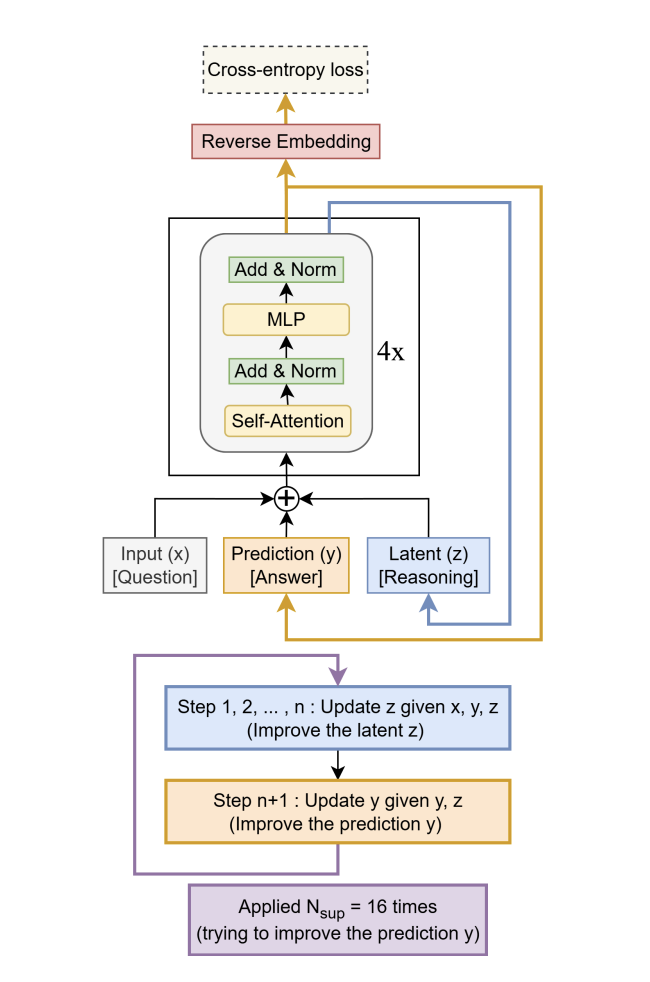
\includegraphics[width=0.75\textwidth]{img/trm_paper.png}
    \caption{Architettura del Tiny Recursive Model (TRM).
        Fonte: \cite{trm}.}
    \label{fig:trm_architecture}
\end{figure}

\clearpage
\newpage
\section{Architettura}

\subsection{Obiettivi progettuali e architettura generale}

L'obiettivo del progetto è stato adattare l'architettura Tiny Recursive Model (TRM) al gioco del Go, realizzando un sistema in grado di prevedere le mosse a partire dallo stato della partita e di utilizzare tali previsioni per giocare autonomamente. Il lavoro non si è limitato all'adattamento del modello neurale, ma ha richiesto la progettazione di un insieme di componenti che ne consentissero l'integrazione in un ambiente di gioco completo.

La TRM costituisce il nucleo neurale del sistema. L'obiettivo è stato mantenerne il meccanismo di ragionamento ricorsivo, intervenendo sulle componenti necessarie per adattarlo al nuovo dominio: la rappresentazione dello stato della scacchiera in ingresso e la produzione delle previsioni in uscita. In particolare, il modello deve associare a ciascuna possibile intersezione del goban un punteggio, considerando anche l'azione di passaggio (\textit{PASS}) tra le mosse disponibili.

Dal punto di vista architetturale, si è scelto di separare la componente neurale dalla gestione delle regole del gioco. La prima si occupa di elaborare le informazioni relative alla partita e stimare le mosse più promettenti; la seconda gestisce lo stato della scacchiera, verifica la legalità delle mosse e applica le conseguenti modifiche alla partita. Questa separazione consente di mantenere distinti il processo di previsione del modello e il funzionamento dell'ambiente di gioco.

Un ulteriore obiettivo è stato supportare entrambe le dimensioni di scacchiera considerate nel progetto, 9×9 e 19×19. Il sistema è stato quindi organizzato in modo da poter utilizzare configurazioni del modello e relativi pesi addestrati per ciascuna dimensione, mantenendo una struttura software condivisa.

Per rendere il sistema concretamente utilizzabile, il modello è stato integrato all'interno di agenti in grado di interagire con l'ambiente di gioco. Questi permettono sia di affrontare una partita contro un giocatore umano, sia di eseguire partite tra agenti autonomi.

È stata inoltre sviluppata un'interfaccia grafica per visualizzare la scacchiera e interagire con il sistema.

Infine, l'architettura prevede la possibilità di estendere la selezione delle mosse attraverso algoritmi di ricerca. In particolare, è stata introdotta un'opzione basata su Negamax, che utilizza le previsioni della TRM per orientare l'esplorazione delle mosse e delle possibili risposte dell'avversario. In questo modo è possibile confrontare la selezione diretta basata sulle previsioni del modello con una strategia che integra anche una fase di ricerca.

Nel complesso, il sistema è stato organizzato in componenti distinte ma integrate: rappresentazione dello stato di gioco, modello neurale, ambiente di gioco, agenti e interfaccia grafica. Questa organizzazione costituisce la base per l'adattamento della TRM al Go e per la successiva valutazione delle diverse strategie di selezione delle mosse.\
\subsection{Adattamento della TRM al gioco del Go}

Per adattare la Tiny Recursive Model al gioco del Go è stato necessario intervenire sulle modalità con cui le informazioni vengono rappresentate e fornite al nucleo ricorsivo. A differenza dei problemi per i quali è stata originariamente sviluppata, il Go presenta uno stato di gioco dinamico, nel quale la disposizione delle pietre cambia progressivamente in seguito alle mosse dei due giocatori.

L'adattamento ha quindi richiesto la progettazione di una rappresentazione in ingresso capace di descrivere lo stato della partita, di un encoder in grado di estrarre le caratteristiche spaziali della scacchiera e di una trasformazione che convertisse tali informazioni nella sequenza di token utilizzata dalla TRM.

\subsubsection{Rappresentazione dello stato del gioco}

La prima modifica riguarda la rappresentazione dello stato del gioco fornita in ingresso al modello. Una semplice rappresentazione della scacchiera corrente permette di descrivere la disposizione delle pietre, ma non contiene informazioni esplicite sulle configurazioni precedenti.

Nel Go, tuttavia, l'evoluzione della scacchiera è importante per interpretare correttamente la situazione corrente. Per questo motivo, si è scelto di utilizzare una rappresentazione composta da sette canali, organizzati come mappe bidimensionali della stessa dimensione della scacchiera.

I primi sei canali descrivono la posizione delle pietre nei tre stati più recenti della partita, distinguendo in ciascuno di essi le pietre del giocatore corrente da quelle dell'avversario. Il settimo canale identifica invece il colore del giocatore che deve effettuare la mossa.

La struttura dell'input è riassunta nella Tabella~\ref{tab:go_input_channels}.

\begin{table}[H]
    \centering
    \begin{tabular}{c|l}
        \textbf{Canale} & \textbf{Informazione rappresentata}          \\
        \hline
        0               & Pietre del giocatore corrente al tempo $T$   \\
        1               & Pietre dell'avversario al tempo $T$          \\
        2               & Pietre del giocatore corrente al tempo $T-1$ \\
        3               & Pietre dell'avversario al tempo $T-1$        \\
        4               & Pietre del giocatore corrente al tempo $T-2$ \\
        5               & Pietre dell'avversario al tempo $T-2$        \\
        6               & Indicatore del colore del giocatore corrente
    \end{tabular}
    \caption{Canali utilizzati per rappresentare lo stato del gioco.}
    \label{tab:go_input_channels}
\end{table}

L'utilizzo di tre configurazioni temporali consente alla rete di ricevere informazioni non soltanto sulla disposizione attuale delle pietre, ma anche sulla sua evoluzione recente. In questo modo, il modello può disporre di un contesto temporale più ampio rispetto a quello ottenibile considerando esclusivamente la scacchiera corrente.

La distinzione tra giocatore corrente e avversario permette inoltre di utilizzare una rappresentazione coerente rispetto al punto di vista del giocatore che deve effettuare la mossa. Questa scelta rende la codifica indipendente dal colore effettivo delle pietre: le informazioni vengono infatti organizzate in base al ruolo dei due giocatori nella posizione considerata.

Infine, l'utilizzo di un canale separato per ciascuna caratteristica consente di mantenere distinte le diverse informazioni fornite al modello, rendendole disponibili come mappe spaziali indipendenti durante la successiva fase di elaborazione.

\subsubsection{Encoder convoluzionale}

Una volta definita la rappresentazione dello stato del gioco, è necessario trasformare le informazioni in ingresso in una rappresentazione adatta al nucleo ricorsivo della TRM.

A questo scopo è stato introdotto un encoder convoluzionale, denominato \texttt{GoEncoder}, che elabora il tensore iniziale attraverso una convoluzione bidimensionale. La scelta di utilizzare una convoluzione, anziché una trasformazione lineare, è legata alla natura spaziale del Go.

La disposizione delle pietre sulla scacchiera presenta infatti relazioni locali particolarmente significative. Adiacenze, libertà e configurazioni tattiche dipendono dalla posizione relativa delle intersezioni e dalle informazioni presenti nelle celle circostanti. Una convoluzione permette di elaborare direttamente queste relazioni, applicando filtri che considerano simultaneamente le informazioni provenienti da regioni locali della scacchiera.

Inoltre, i pesi dei filtri convoluzionali vengono condivisi tra le diverse posizioni. Questo consente di applicare gli stessi criteri di estrazione delle caratteristiche in ogni regione del goban, indipendentemente dalla posizione in cui si trovano le configurazioni considerate.

L'encoder utilizza una convoluzione 2D con kernel di dimensione $3 \times 3$ e padding pari a 1. Il kernel permette di considerare, per ciascuna posizione, anche le intersezioni immediatamente circostanti, mentre il padding mantiene invariate le dimensioni spaziali della scacchiera dopo l'operazione.

Alla convoluzione seguono un livello di Batch Normalization e una funzione di attivazione ReLU. La Batch Normalization contribuisce a rendere più stabile la distribuzione delle attivazioni durante l'addestramento, mentre ReLU introduce una non linearità necessaria per consentire alla rete di apprendere rappresentazioni più articolate.

Il numero di canali in uscita dalla convoluzione è fissato a 256, in modo da ottenere una rappresentazione con la stessa dimensione nascosta utilizzata dal nucleo della TRM. Il passaggio complessivo può essere rappresentato come segue:

\[
    [B, 7, N, N]
    \longrightarrow
    [B, 256, N, N]
\]

dove $B$ indica la dimensione del batch e $N$ la dimensione della scacchiera, pari a 9 oppure 19.

La scelta di mantenere invariate le dimensioni spaziali consente di conservare una corrispondenza tra le posizioni della scacchiera originale e quelle della rappresentazione ottenuta dall'encoder.

Ogni intersezione dispone quindi di un vettore di 256 caratteristiche, che costituisce la base per la successiva trasformazione in sequenza.

\subsubsection{Codifica posizionale e trasformazione in sequenza}

Il nucleo della TRM elabora le informazioni attraverso una rappresentazione sequenziale.
È quindi necessario convertire l'output bidimensionale dell'encoder in una sequenza di token, mantenendo al tempo stesso l'informazione relativa alla posizione delle intersezioni sulla scacchiera.

A partire dal tensore prodotto dalla convoluzione, le due dimensioni spaziali vengono appiattite in un'unica dimensione. Il tensore viene successivamente trasposto per ottenere una sequenza nella quale ciascun elemento rappresenta una singola intersezione del goban.

La trasformazione può essere descritta come:

\[
    [B, 256, N, N]
    \longrightarrow
    [B, N^2, 256]
\]

Il risultato è una sequenza composta da $N^2$ token, ciascuno caratterizzato da un vettore di dimensione 256. In questo modo, ogni posizione della scacchiera viene associata a una rappresentazione che raccoglie le caratteristiche estratte dall'encoder.

La trasformazione in sequenza comporta tuttavia la perdita della disposizione bidimensionale esplicita delle intersezioni. Per permettere al modello di distinguere le diverse posizioni, viene quindi aggiunto un embedding posizionale appreso, rappresentato da una matrice di parametri addestrabili con dimensione $N^2 \times 256$.

L'embedding viene sommato alla rappresentazione di ciascun token, introducendo informazioni sulla sua posizione originale all'interno della scacchiera. Questa scelta permette al nucleo della TRM di distinguere intersezioni che, pur presentando caratteristiche simili, occupano posizioni differenti.

È importante distinguere questa codifica posizionale assoluta dagli eventuali Rotary Positional Embeddings (RoPE) utilizzati all'interno del meccanismo di attenzione.
Nel progetto, l'embedding assoluto viene aggiunto direttamente dall'encoder, mentre l'utilizzo di RoPE è opzionale e controllato separatamente dalla configurazione del modello.

Pertanto, l'impostazione \texttt{pos\_encodings="none"} disabilita l'impiego di RoPE, ma non elimina l'embedding posizionale appreso dall'encoder.

Al termine di questa fase, la rappresentazione della scacchiera è stata convertita in una sequenza di token compatibile con il nucleo ricorsivo della TRM, mantenendo sia le caratteristiche estratte dalle configurazioni locali sia le informazioni relative alla posizione delle singole intersezioni.
\clearpage
\newpage
\section{Implementazione}

\subsection{Organizzazione del progetto}

Il progetto è stato organizzato in moduli Python distinti, ciascuno responsabile di una specifica parte del sistema. Questa suddivisione consente di separare la gestione delle regole del gioco, l'elaborazione neurale, la selezione delle mosse e l'interazione con l'utente, facilitando lo sviluppo e la manutenzione delle singole componenti.

Il codice relativo al modello è raccolto nella cartella \texttt{models/}, mentre i moduli dedicati all'ambiente di gioco, agli agenti e all'interfaccia grafica si trovano nella cartella principale del progetto \texttt{TRM/}. Sono inoltre presenti script e strumenti dedicati alla preparazione dei dataset, all'addestramento e alla valutazione dei modelli.

La Tabella~\ref{tab:project_modules} riassume le responsabilità dei principali moduli Python utilizzati nell'implementazione.

\begin{table}[H]
    \centering
    \begin{tabular}{p{5.0cm}|p{8cm}}
        \textbf{Modulo}                     & \textbf{Responsabilità}                                                                                                            \\
        \hline
        \texttt{game\_env.py}               & Gestione dello stato della partita, applicazione delle regole del Go, verifica della legalità delle mosse e calcolo del punteggio. \\
        \texttt{models/go\_encoder.py}      & Trasformazione dello stato della scacchiera in una sequenza di rappresentazioni vettoriali utilizzabili dalla TRM.                 \\
        \texttt{models/go\_trm.py}          & Implementazione del nucleo ricorsivo della rete e aggiornamento delle rappresentazioni latenti.                                    \\
        \texttt{models/go\_model.py}        & Assemblaggio delle componenti del modello, integrando il nucleo TRM e la Policy Head.                                              \\
        \texttt{models/go\_policy\_head.py} & Conversione delle rappresentazioni prodotte dalla TRM nei logits associati alle mosse sulla scacchiera e all'azione PASS.          \\
        \texttt{agents.py}                  & Caricamento dei checkpoint, esecuzione del modello in inferenza, applicazione dei vincoli di legalità e selezione della mossa.     \\
        \texttt{negamax.py}                 & Implementazione della ricerca Negamax con potatura alpha-beta, utilizzando la policy della TRM per ordinare le mosse candidate.    \\
        \texttt{app.py}                     & Realizzazione dell'interfaccia grafica tramite Pygame e gestione delle partite tra giocatore umano e agenti automatici.            \\
    \end{tabular}
    \caption{Principali moduli Python e relative responsabilità.}
    \label{tab:project_modules}
\end{table}

Il modulo \texttt{game\_env.py} costituisce il riferimento per la gestione delle regole del gioco. È responsabile della rappresentazione della scacchiera, dell'applicazione delle mosse e del controllo della loro legalità. In questo modo, sia gli agenti automatici sia l'interfaccia grafica possono interagire con la partita attraverso un'unica implementazione dell'ambiente, senza dover replicare la logica delle regole.

Le componenti del modello neurale sono invece raccolte nella cartella \texttt{models/}. Il modulo \texttt{go\_encoder.py} prepara la rappresentazione dello stato del gioco, mentre \texttt{go\_trm.py} implementa il processo di ragionamento ricorsivo. Il modulo \texttt{go\_policy\_head.py} elabora le rappresentazioni ottenute per produrre i punteggi associati alle azioni disponibili. Queste componenti vengono integrate da \texttt{go\_model.py}, che definisce il modello completo utilizzato nelle fasi di addestramento e inferenza.

Il modulo \texttt{agents.py} si occupa di utilizzare il modello addestrato durante una partita. In particolare, carica i pesi salvati nel checkpoint, prepara gli input a partire dallo stato dell'ambiente e gestisce la selezione delle mosse, tenendo conto delle azioni legali. All'interno dello stesso modulo è inoltre definito l'agente umano, utilizzato per consentire l'interazione tramite interfaccia grafica.

La ricerca opzionale delle mosse è implementata separatamente in \texttt{negamax.py}.
Questa scelta permette di affiancare alla selezione diretta basata sulla policy una strategia di ricerca, senza modificare il modello neurale o il relativo processo di addestramento.

Il modulo \texttt{app.py}, infine, integra le diverse componenti e fornisce l'interfaccia grafica attraverso cui è possibile configurare e avviare le partite.

La separazione tra questi moduli permette quindi di mantenere indipendenti le principali responsabilità del sistema, favorendo il riutilizzo delle componenti e consentendo di modificare o valutare una parte dell'implementazione senza dover intervenire necessariamente sulle altre.
\subsection{Preparazione del dataset}

Le partite utilizzate per l'addestramento, disponibili in formato SGF, vengono elaborate per ottenere un dataset di esempi supervisionati. Ogni esempio è costituito dalla rappresentazione dello stato della scacchiera in un determinato momento della partita e dalla mossa successivamente effettuata dal giocatore di turno.

La pipeline è implementata principalmente nei moduli \texttt{go\_preprocessing.py} e \texttt{go\_dataset.py} e comprende il parsing delle partite, l'estrazione delle feature e delle mosse target, la suddivisione dei dati e il loro salvataggio.

\subsubsection{Lettura delle partite ed estrazione degli esempi}

La lettura dei file SGF viene effettuata mediante la libreria \texttt{sgfmill}, utilizzata per ricostruire la sequenza delle mosse. Durante il parsing viene verificata la dimensione della scacchiera, così da escludere le partite non compatibili con la configurazione in elaborazione.

Per ciascuna partita, il programma ricostruisce progressivamente lo stato del goban. Prima di applicare ogni mossa vengono memorizzati la configurazione corrente della scacchiera e il colore del giocatore di turno: queste informazioni costituiscono rispettivamente l'input e l'etichetta dell'esempio.

La mossa target viene codificata mediante un indice intero. Le intersezioni assumono valori compresi tra \(0\) e \(N^2-1\), mentre l'azione \textit{PASS} è rappresentata dall'indice \(N^2\), dove \(N\) indica la dimensione della scacchiera.

Durante la ricostruzione vengono controllate anche le mosse illegali. Gli esempi corrispondenti a mosse non applicabili vengono esclusi e la partita viene segnalata come non valida.

Una gestione specifica riguarda la conclusione delle partite: due mosse \textit{PASS} consecutive determinano la terminazione del gioco, ma alcuni file SGF possono non riportarle entrambe esplicitamente. Quando il risultato registrato è compatibile con una conclusione basata sul punteggio, il preprocessing ricostruisce gli eventuali PASS mancanti, evitando di introdurre mosse artificiali nei casi di abbandono o conclusione per tempo.

\subsubsection{Estrazione delle feature}

La funzione \texttt{extract\_features()} converte lo stato della partita in un tensore numerico di forma \(7\times N\times N\), coerente con l'input richiesto dal modello.

La rappresentazione considera tre configurazioni temporali della scacchiera, quella corrente (\(T\)) e le due precedenti (\(T-1\) e \(T-2\)). Per ciascuna vengono utilizzati due canali che distinguono le pietre del giocatore corrente da quelle dell'avversario; un ulteriore canale identifica il colore del giocatore di turno.

I primi sei canali sono mappe binarie, mentre il settimo assume valore costante su tutta la scacchiera: 1 per il Nero e 0 per il Bianco.

La costruzione dei canali avviene rispetto al giocatore corrente, mantenendo una prospettiva uniforme indipendentemente dal colore che deve effettuare la mossa. Il principio di implementazione è il seguente:

\begin{verbatim}
player_channel = history_idx * 2
opponent_channel = history_idx * 2 + 1

tensor[player_channel] = board_array == current_color
tensor[opponent_channel] = board_array == opposite_color(current_color)
\end{verbatim}

Il tensore risultante viene convertito in formato \texttt{float32}, mentre la mossa target viene memorizzata separatamente come indice intero. Ogni esempio presenta pertanto un input di forma \([7,N,N]\) e un'etichetta scalare.

\subsubsection{Suddivisione del dataset}

Gli esempi vengono organizzati in tre insiemi: training, validation e test, secondo una proporzione rispettivamente pari all'80\%, 10\% e 10\%.

La suddivisione avviene a livello di partita e non di singola posizione. Questa scelta evita che esempi appartenenti alla stessa partita siano distribuiti tra insiemi differenti, riducendo il rischio di data leakage e rendendo più significativa la valutazione della capacità di generalizzazione.

La selezione viene effettuata in maniera riproducibile mediante un generatore casuale inizializzato con seed pari a 42.

Per il dataset 19$\times$19, considerate le dimensioni dell'archivio originale, è inoltre possibile limitare il numero di partite elaborate. Nella configurazione utilizzata sono state selezionate al massimo 10.000 partite, prima della suddivisione nei tre insiemi. Anche questa selezione è deterministica.

\subsubsection{Data augmentation mediante simmetrie \texorpdfstring{\(D_4\)}{D4}}

Durante l'addestramento viene applicata una tecnica di \textit{data augmentation} basata sulle otto simmetrie del gruppo diedrale \(D_4\), corrispondenti alle quattro rotazioni di \(0^\circ\), \(90^\circ\), \(180^\circ\) e \(270^\circ\) e alle rispettive riflessioni.

Queste trasformazioni mantengono inalterate le relazioni tra le intersezioni e permettono di ottenere configurazioni equivalenti del gioco con orientamenti differenti.

La trasformazione viene applicata sia alle feature sia alla mossa target, che deve essere rimappata nella nuova posizione. L'azione \textit{PASS}, non essendo associata a un'intersezione, rimane invece invariata.

L'implementazione è contenuta nella funzione \texttt{apply\_board\_symmetry()} del modulo \texttt{go\_dataset.py}. A ogni campione viene applicata casualmente una delle otto trasformazioni durante il caricamento, senza generare preventivamente copie aggiuntive del dataset.

La data augmentation è attiva esclusivamente per il training; validation e test mantengono la rappresentazione originale, garantendo la riproducibilità delle metriche.

\subsubsection{Salvataggio e caricamento dei dati}

I dataset vengono salvati in formato NumPy, attraverso il formato compresso \texttt{NPZ} oppure mediante file \texttt{NPY}, utilizzati nelle configurazioni principali per gestire gli insiemi di dimensioni maggiori.

In quest'ultimo caso, ciascun insieme contiene due file:

\begin{itemize}
    \item \texttt{X.npy}, contenente i tensori delle feature in formato \texttt{float32};
    \item \texttt{y.npy}, contenente gli indici delle mosse target in formato \texttt{int64}.
\end{itemize}

Per evitare di caricare interamente in memoria dataset particolarmente grandi, viene utilizzato il \textit{memory mapping} di NumPy:

\begin{verbatim}
self.X = np.load("X.npy", mmap_mode="r")
self.y = np.load("y.npy", mmap_mode="r")
\end{verbatim}

Questa modalità consente di accedere ai dati direttamente dai file, caricando in memoria soltanto le porzioni necessarie. Il vantaggio è particolarmente rilevante per il dataset 19$\times$19.

Durante l'addestramento, la classe \texttt{GoDataset} gestisce l'accesso ai campioni, mentre i \textit{DataLoader} di PyTorch organizzano il caricamento in batch. Le trasformazioni casuali vengono applicate esclusivamente agli esempi di training.

La pipeline produce quindi tre insiemi distinti, pronti per l'addestramento e la valutazione, mantenendo la stessa struttura logica per entrambe le dimensioni di scacchiera.

\subsection{Implementazione del modello}

Il modello è implementato mediante PyTorch e organizzato in tre componenti principali: encoder convoluzionale, nucleo ricorsivo e Policy Head. Queste componenti sono definite in moduli separati e integrate dalla classe \texttt{GoTRMModel}, implementata in \texttt{go\_model.py}.

\subsubsection{Encoder convoluzionale}

L'encoder è implementato nella classe \texttt{GoEncoder}, definita in \texttt{go\_encoder.py}. Il blocco convoluzionale iniziale è costituito da una convoluzione bidimensionale, seguita da Batch Normalization e ReLU:

\begin{lstlisting}[language=Python, caption={Definizione del blocco convoluzionale di GoEncoder}, label={lst:go_encoder}]
self.conv_stem = nn.Sequential(
    nn.Conv2d(in_channels, hidden_size,
              kernel_size=3, padding=1, bias=False),
    nn.BatchNorm2d(hidden_size),
    nn.ReLU()
)
\end{lstlisting}

La convoluzione trasforma i sette canali iniziali in 256 mappe di caratteristiche, mantenendo invariate le dimensioni spaziali grazie al kernel \(3\times3\) e al padding pari a 1.

Il risultato viene successivamente convertito nella sequenza di token richiesta dal nucleo ricorsivo. Le dimensioni spaziali vengono appiattite e riordinate, mentre a ciascun token viene sommato il corrispondente embedding posizionale apprendibile:

\begin{lstlisting}[language=Python, caption={Conversione delle mappe convoluzionali in una sequenza}, label={lst:go_encoder_sequence}]
x = self.conv_stem(x)

batch_size = x.size(0)
x = x.view(batch_size, x.size(1), -1)
x = x.transpose(1, 2)

x = x + self.pos_embedding
\end{lstlisting}

L'output assume forma \([B,N^2,256]\), dove \(B\) indica la dimensione del batch e \(N\) quella della scacchiera.

\subsubsection{Nucleo ricorsivo}

Il nucleo è implementato nel modulo \texttt{go\_trm.py}, che contiene le classi dedicate alla configurazione, ai blocchi di elaborazione e alla gestione degli stati ricorsivi.

Gli stati \(z_H\) e \(z_L\) sono rappresentati mediante tensori di forma \([B,N^2,256]\). La loro inizializzazione e il ripristino sono gestiti rispettivamente dai metodi \texttt{empty\_carry()} e \texttt{reset\_carry()}.

Il metodo \texttt{forward()} coordina gli aggiornamenti ricorsivi, reinserendo la rappresentazione prodotta dall'encoder durante gli aggiornamenti di \(z_L\):

\begin{lstlisting}[language=Python, caption={Aggiornamento ricorsivo degli stati latenti}, label={lst:trm_cycles}]
input_embeddings = self.go_encoder(batch["inputs"])

z_H, z_L = carry.z_H, carry.z_L

with torch.no_grad():
    for _ in range(self.config.H_cycles - 1):
        for _ in range(self.config.L_cycles):
            z_L = self.L_level(z_L, z_H + input_embeddings)
        z_H = self.L_level(z_H, z_L)

for _ in range(self.config.L_cycles):
    z_L = self.L_level(z_L, z_H + input_embeddings)
z_H = self.L_level(z_H, z_L)
\end{lstlisting}

Gli aggiornamenti utilizzano lo stesso modulo \texttt{L\_level}, condividendone i parametri tra i due stati e le diverse iterazioni.

La gestione del gradiente costituisce un aspetto rilevante dell'implementazione: i primi \(H\_cycles-1\) cicli vengono eseguiti mediante \texttt{torch.no\_grad()}, mentre il ciclo finale mantiene attivo il calcolo necessario alla retropropagazione. Al termine, gli stati aggiornati vengono salvati nella struttura \texttt{carry}, utilizzando \texttt{detach()} per separarli dal grafo computazionale.

Il numero di aggiornamenti è determinato dai parametri \texttt{H\_cycles} e \texttt{L\_cycles}, consentendo di modificare la profondità ricorsiva attraverso la configurazione senza intervenire sul codice del modello.

\subsubsection{Policy Head}

La classe \texttt{GoPolicyHead}, definita in \texttt{go\_policy\_head.py}, riceve la sequenza prodotta dal nucleo ricorsivo e genera i logits associati alle azioni.

Per le intersezioni viene utilizzato un MLP condiviso tra tutti i token:

\begin{lstlisting}[language=Python, caption={MLP per la previsione delle mosse sul tabellone}, label={lst:policy_board}]
self.board_mlp = nn.Sequential(
    nn.Linear(hidden_size, hidden_size // 2),
    nn.ReLU(),
    nn.Linear(hidden_size // 2, 1)
)
\end{lstlisting}

Il ramo dedicato a \textit{PASS} utilizza invece una rappresentazione globale, ottenuta mediante media delle rappresentazioni latenti lungo la dimensione della sequenza:

\begin{lstlisting}[language=Python, caption={Generazione del logit PASS}, label={lst:policy_pass}]
global_features = x.mean(dim=1)
pass_logit = self.pass_mlp(global_features)
\end{lstlisting}

I risultati vengono infine concatenati per produrre un vettore di \(N^2+1\) valori:

\begin{lstlisting}[language=Python, caption={Composizione dell'output della Policy Head}, label={lst:policy_output}]
board_logits = self.board_mlp(x).squeeze(-1)
logits = torch.cat([board_logits, pass_logit], dim=-1)
return logits
\end{lstlisting}

I primi \(N^2\) valori corrispondono alle intersezioni, mentre l'ultimo rappresenta l'azione \textit{PASS}. I valori ottenuti sono logits non normalizzati e vengono convertiti in probabilità soltanto durante la fase di inferenza.

\paragraph{Integrazione dei componenti}

La classe \texttt{GoTRMModel}, definita in \texttt{go\_model.py}, integra encoder, nucleo ricorsivo e Policy Head. Il metodo \texttt{forward()} coordina il passaggio delle rappresentazioni tra i moduli:

\begin{lstlisting}[language=Python, caption={Integrazione tra nucleo ricorsivo e Policy Head}, label={lst:go_model}]
carry = self.trm.initial_carry(batch_dict)
carry, hidden_features = self.trm(carry, batch_dict)
return self.policy_head(hidden_features)
\end{lstlisting}

In questo modo, le procedure di addestramento e inferenza possono utilizzare il modello completo attraverso un'unica interfaccia, senza dover gestire separatamente le singole componenti.

\subsection{Processo di addestramento}

L'addestramento del modello avviene mediante apprendimento supervisionato, utilizzando le posizioni e le mosse estratte dalle partite SGF durante la fase di preparazione del dataset. Per ciascun esempio, il modello riceve la rappresentazione dello stato corrente della scacchiera e deve prevedere la mossa successivamente eseguita nella partita originale.

L'obiettivo è quindi apprendere una \textit{policy}, ossia una distribuzione di preferenza sulle possibili azioni, attraverso il confronto tra le predizioni della rete e le mosse presenti nel dataset.

La procedura è implementata nel file \texttt{train.py} e utilizza PyTorch per la gestione del modello, il calcolo della funzione di perdita e l'aggiornamento dei parametri.

\subsubsection{Apprendimento supervisionato e funzione di perdita}

Durante l'addestramento, ogni batch contiene un insieme di rappresentazioni della scacchiera e le corrispondenti mosse target. Le mosse sono codificate come indici interi: un valore compreso tra \(0\) e \(N^2-1\) identifica un'intersezione della scacchiera, mentre il valore \(N^2\) rappresenta l'azione \textit{PASS}.

Il modello restituisce, per ogni esempio, un vettore di \(N^2+1\) logits, uno per ciascuna azione possibile. Questi valori vengono confrontati con le mosse target mediante la funzione \texttt{CrossEntropyLoss} di PyTorch:

\begin{lstlisting}[language=Python, caption={Definizione della funzione di perdita}, label={lst:training_loss}]
criterion = nn.CrossEntropyLoss()

logits = model(x_batch)
loss = criterion(logits, y_batch)
\end{lstlisting}

La Cross Entropy Loss misura la discrepanza tra le predizioni del modello e le classi corrette. In particolare, penalizza le predizioni che assegnano una probabilità ridotta alla mossa effettivamente presente nel dataset.

La funzione opera direttamente sui logits, applicando internamente la normalizzazione necessaria al calcolo della perdita. Non è quindi necessario applicare esplicitamente una softmax prima di passarle le predizioni.

\subsubsection{Ottimizzazione dei parametri e learning rate}

L'aggiornamento dei pesi della rete è affidato all'ottimizzatore \texttt{AdamW}, che combina il metodo Adam con una gestione separata del decadimento dei pesi (\textit{weight decay}).

La configurazione utilizzata prevede un learning rate iniziale pari a \(10^{-4}\), un weight decay pari a \(10^{-4}\) e i coefficienti \(\beta_1=0.9\) e \(\beta_2=0.95\).

Il processo di ottimizzazione viene eseguito attraverso le operazioni standard di PyTorch:

\begin{lstlisting}[language=Python, caption={Aggiornamento dei parametri durante il training}, label={lst:training_step}]
optimizer.zero_grad(set_to_none=True)

logits = model(x_batch)
loss = criterion(logits, y_batch)

loss.backward()
optimizer.step()
scheduler.step()
\end{lstlisting}

A ogni iterazione vengono inizialmente azzerati i gradienti accumulati, quindi viene eseguito il passaggio in avanti del modello e calcolata la funzione di perdita. La chiamata a \texttt{backward()} calcola i gradienti rispetto ai parametri apprendibili, mentre \texttt{optimizer.step()} aggiorna i pesi della rete.

Dopo ogni aggiornamento dei parametri viene eseguito anche lo scheduler del learning rate.

La variazione del learning rate segue una strategia composta da due fasi: un periodo iniziale di \textit{warmup}, seguito da un decadimento secondo una funzione coseno (\textit{cosine decay}).

Durante il warmup, il learning rate aumenta progressivamente fino al valore iniziale previsto. Questa fase consente di evitare aggiornamenti troppo ampi nelle prime iterazioni dell'addestramento. Successivamente, il learning rate diminuisce gradualmente secondo una curva coseno, fino a raggiungere un valore minimo configurato.

Nel progetto, lo scheduler è implementato mediante \texttt{LambdaLR} e viene aggiornato a ogni passo dell'ottimizzatore, anziché una sola volta per epoca. La configurazione predefinita prevede 2000 passi di warmup, un learning rate iniziale di \(10^{-4}\) e un valore minimo di \(10^{-5}\).

\subsubsection{Validazione e selezione del modello}

Al termine di ogni epoca, il modello viene valutato sul validation set, che non viene utilizzato per aggiornare i parametri della rete. Questa fase permette di monitorare la capacità del modello di generalizzare a posizioni non utilizzate durante l'addestramento.

La valutazione viene eseguita disabilitando il calcolo dei gradienti e misurando tre metriche principali:

\begin{itemize}
    \item \textbf{Validation Loss}: valore medio della Cross Entropy Loss sugli esempi di validazione.
    \item \textbf{Top-1 Accuracy}: percentuale di esempi per i quali la mossa target corrisponde alla predizione con il logit più alto.
    \item \textbf{Top-3 Accuracy}: percentuale di esempi per i quali la mossa target compare tra le tre azioni con i logits più elevati.
\end{itemize}

La selezione del modello migliore si basa sulla Validation Loss. Quando il valore ottenuto è inferiore al minimo registrato nelle epoche precedenti, i pesi correnti vengono salvati come nuovo modello migliore.

Questa scelta permette di selezionare il checkpoint in base alla qualità complessiva delle predizioni, anziché considerare esclusivamente la percentuale di mosse corrette al primo posto.

\subsubsection{Salvataggio dei checkpoint}

Durante l'addestramento vengono gestiti due checkpoint distinti, con finalità differenti:

\begin{itemize}
    \item \texttt{best\_model.pt}: contiene i pesi del modello che ha ottenuto la migliore Validation Loss, insieme alla configurazione necessaria per ricostruire l'architettura. Include inoltre alcune informazioni relative all'addestramento e alle metriche di validazione. È il checkpoint destinato principalmente al caricamento del modello durante l'inferenza.

    \item \texttt{latest\_model.pt}: contiene lo stato completo dell'addestramento, comprendendo i pesi del modello, lo stato dell'ottimizzatore, quello dello scheduler, l'epoca e il passo raggiunti, la configurazione e gli stati dei generatori casuali. Viene utilizzato per riprendere un addestramento interrotto.
\end{itemize}

Il checkpoint \texttt{latest\_model.pt} viene aggiornato periodicamente, ogni 500 passi di ottimizzazione nella configurazione predefinita, e al termine di ogni epoca. Il checkpoint \texttt{best\_model.pt} viene invece aggiornato soltanto quando la Validation Loss migliora rispetto al valore migliore precedentemente registrato.

Il salvataggio viene effettuato inizialmente su un file temporaneo, che viene successivamente rinominato nella destinazione definitiva. Questa procedura riduce il rischio di lasciare un checkpoint incompleto in caso di interruzione durante la scrittura.

\subsubsection{Ripresa dell'addestramento}

Per consentire la ripresa di un addestramento interrotto viene implementato il parametro \texttt{--resume}, che permette di ripartire dallo stato registrato in \texttt{latest\_model.pt}.

A differenza del semplice caricamento dei pesi, questa procedura ripristina anche lo stato dell'ottimizzatore e dello scheduler. In questo modo vengono conservate le informazioni accumulate durante le iterazioni precedenti, evitando di iniziare nuovamente l'ottimizzazione da una condizione iniziale.

Vengono inoltre ripristinati il numero di epoca, il passo raggiunto all'interno dell'epoca e gli stati dei generatori casuali utilizzati da Python, NumPy e PyTorch. Quest'ultimo aspetto consente di mantenere la continuità del processo, anche rispetto all'ordine dei campioni e alle operazioni casuali impiegate durante il training.

La configurazione predefinita di \texttt{--resume} ripristina anche il learning rate e lo scheduler dal checkpoint, consentendo di proseguire il piano di ottimizzazione originale. È tuttavia possibile specificare esplicitamente un nuovo learning rate: in questo caso viene mantenuto lo stato accumulato dall'ottimizzatore, ma viene avviata una nuova fase di cosine decay a partire dal valore indicato, senza ripetere il warmup.

Il meccanismo di ripresa permette quindi sia di continuare un addestramento interrotto mantenendo la configurazione precedente, sia di modificare esplicitamente il learning rate quando si desidera adattare la fase finale dell'ottimizzazione.

\paragraph{Sintesi del ciclo di addestramento}

Il processo complessivo può essere riassunto attraverso il seguente pseudocodice:

\begin{lstlisting}[language=Python, caption={Schema semplificato del processo di addestramento}, label={lst:training_loop}]
for epoch in range(start_epoch, epochs + 1):

    model.train()

    for x_batch, y_batch in train_loader:

        optimizer.zero_grad()
        logits = model(x_batch)
        loss = criterion(logits, y_batch)

        loss.backward()
        optimizer.step()
        scheduler.step()

        if checkpoint_interval:
            save_latest_checkpoint()

    val_loss, val_top1, val_top3 = evaluate(model, val_loader)

    if val_loss < best_val_loss:
        best_val_loss = val_loss
        save_best_checkpoint()

    save_latest_checkpoint()
\end{lstlisting}

Al termine del processo, il file \texttt{best\_model.pt} contiene la versione del modello selezionata sulla base delle prestazioni ottenute sul validation set. I relativi pesi vengono successivamente utilizzati per le prove di inferenza e per la valutazione delle prestazioni nel gioco del Go.

\subsection{Inferenza e selezione delle mosse}

Durante una partita, il modello viene utilizzato per individuare la mossa da eseguire a partire dallo stato corrente della scacchiera. Questa fase è gestita dalla classe \texttt{TRMAgent}, implementata nel file \texttt{agents.py}.

A differenza dell'addestramento, durante l'inferenza i parametri della rete rimangono invariati. L'agente carica il modello, prepara l'input, esegue il forward pass e trasforma le predizioni in un'azione compatibile con le regole del gioco.

\subsubsection{Caricamento del modello e preparazione dell'input}

All'inizializzazione, l'agente carica il checkpoint \texttt{best\_model.pt}, dal quale recupera la configurazione necessaria a ricostruire il modello e i relativi pesi:

\begin{lstlisting}[language=Python, caption={Caricamento del modello dal checkpoint}, label={lst:inference_load}]
checkpoint = torch.load(checkpoint_path, map_location=self.device)
config_dict = checkpoint["config_dict"]

self.model = GoTRMModel(config_dict).to(self.device)
self.model.load_state_dict(checkpoint["model_state_dict"])
self.model.eval()
\end{lstlisting}

Il modello viene trasferito sul dispositivo disponibile, selezionato tra CUDA, Apple MPS e CPU, e impostato in modalità valutazione.

Prima dell'inferenza, il metodo \texttt{\_extract\_features()} costruisce il tensore di input a partire dallo stato mantenuto dall'ambiente. La rappresentazione è coerente con quella utilizzata durante il training e presenta forma \([1,7,N,N]\).

L'esecuzione del modello avviene senza calcolo dei gradienti:

\begin{lstlisting}[language=Python, caption={Esecuzione del forward pass durante l'inferenza}, label={lst:inference_forward}]
x = self._extract_features(env)

with torch.inference_mode():
    logits = self.model(x).squeeze(0)
\end{lstlisting}

Il risultato è un vettore di \(N^2+1\) logits, corrispondenti alle intersezioni e all'azione \textit{PASS}.

\subsubsection{Filtraggio delle mosse illegali}

Prima della selezione, è necessario escludere le azioni non consentite dalle regole del Go. L'agente richiede all'ambiente una maschera mediante il metodo \texttt{get\_legal\_moves\_mask()}, che restituisce un vettore booleano della stessa dimensione dei logits.

Le azioni illegali vengono escluse sostituendo i rispettivi valori con \(-\infty\):

\begin{lstlisting}[language=Python, caption={Mascheramento delle mosse illegali}, label={lst:legal_mask}]
masked_logits = logits.masked_fill(
    ~legal_mask,
    float("-inf")
)
\end{lstlisting}

In questo modo, dopo la normalizzazione, tali azioni ricevono probabilità nulla e non possono essere selezionate. La verifica rimane delegata all'ambiente, che costituisce l'unico riferimento per la legalità delle mosse.

\subsubsection{Penalizzazione della mossa PASS}

Per ridurre la tendenza del modello a interrompere prematuramente la partita, durante l'inferenza può essere applicata una penalizzazione al logit associato a \textit{PASS}.

La configurazione predefinita prevede una penalità pari a \(3.5\), applicata quando il numero di pietre presenti sulla scacchiera è inferiore a 16:

\begin{lstlisting}[language=Python, caption={Penalizzazione del logit PASS}, label={lst:pass_penalty}]
if occupied_stones < before_stones:
    adjusted_logits = logits.clone()
    adjusted_logits[-1] -= penalty
\end{lstlisting}

La penalizzazione interviene esclusivamente sul valore di \textit{PASS}, non modifica i pesi del modello e può essere regolata o disabilitata attraverso i parametri di configurazione.

\subsubsection{Conversione in probabilità e selezione della mossa}

Dopo il filtraggio e l'eventuale penalizzazione, i logits vengono convertiti in probabilità mediante softmax:

\[
    P(a_i) =
    \frac{\exp(l_i)}
    {\sum_{j \in A_{\mathrm{legali}}}\exp(l_j)}
\]

dove \(A_{\mathrm{legali}}\) rappresenta l'insieme delle azioni consentite.

La selezione non consiste necessariamente nell'individuare l'azione con probabilità massima. L'agente considera infatti tutte le mosse la cui probabilità risulta sufficientemente vicina a quella della migliore candidata.

Indicando con \(p_{\max}\) la probabilità massima, viene definita una soglia pari al 98\% di tale valore:

\[
    p_{\mathrm{soglia}}=0.98\cdot p_{\max}
\]

L'insieme delle mosse candidate è quindi:

\[
    A_{\mathrm{candidate}} =
    \left\{
    a_i \in A_{\mathrm{legali}}
    \mid P(a_i)\geq 0.98\cdot p_{\max}
    \right\}
\]

La mossa viene infine estratta uniformemente da questo insieme:

\[
    a_{\mathrm{scelta}}\sim
    \operatorname{Uniforme}(A_{\mathrm{candidate}})
\]

La tolleranza del 2\% è relativa alla probabilità massima e non rappresenta una differenza assoluta di due punti percentuali. In presenza di più azioni con probabilità simili, l'agente introduce quindi una componente stocastica, evitando di selezionare sistematicamente la stessa mossa.

La procedura è implementata nella funzione \texttt{select\_near\_best\_action()}. L'azione restituita viene infine passata all'ambiente, che ne gestisce l'esecuzione e l'aggiornamento dello stato della partita.

\subsection{Implementazione della ricerca Negamax}

Per affiancare alla selezione diretta delle mosse una componente di ricerca, è stato implementato un agente basato sull'algoritmo Negamax con potatura alpha-beta. Questa modalità non sostituisce la rete TRM, ma la utilizza come supporto per individuare e ordinare le mosse da esplorare.

La TRM continua infatti a generare una distribuzione di probabilità sulle azioni possibili, mentre Negamax utilizza tali informazioni per costruire un albero di ricerca composto da sequenze alternative di mosse. L'obiettivo è valutare non soltanto la mossa immediatamente più probabile, ma anche le possibili risposte dell'avversario e le conseguenze delle proprie scelte.

\subsubsection{Generazione e ordinamento delle mosse candidate}

A ogni nodo dell'albero, l'agente interroga la policy TRM per ottenere le probabilità associate alle azioni disponibili. Le mosse illegali vengono escluse utilizzando la maschera fornita dall'ambiente di gioco.

Le mosse legali vengono quindi ordinate in base alla probabilità assegnata dalla rete e vengono selezionate le prime $K$, dove $K$ rappresenta il numero massimo di candidate considerate per ciascun nodo. Questo limite consente di contenere il numero di rami esplorati, evitando di dover analizzare tutte le mosse possibili in ogni posizione.

La selezione non si basa esclusivamente sulle indicazioni della rete. Vengono infatti aggiunte alcune mosse tatticamente rilevanti, anche quando la loro probabilità è inferiore rispetto a quella delle candidate selezionate inizialmente. In particolare, vengono considerate le libertà delle catene di pietre che si trovano in atari, così da includere le possibili mosse di cattura o di salvataggio.

Anche la mossa PASS può essere inclusa tra le candidate: viene considerata quando rientra tra le azioni con probabilità più elevata oppure quando l'avversario ha già effettuato un PASS, situazione nella quale è necessario valutare anche la possibilità di terminare la partita.

Le mosse candidate vengono infine ordinate, dando precedenza a quelle tattiche e utilizzando successivamente la probabilità della policy come criterio di ordinamento. Questo approccio permette di combinare le indicazioni apprese dalla rete con alcune informazioni tattiche ricavate direttamente dalla configurazione della scacchiera.

\subsubsection{Ricerca a profondità limitata e potatura alpha-beta}

Una volta individuate le mosse candidate, l'agente esplora ricorsivamente le possibili sequenze di gioco attraverso l'algoritmo Negamax. La ricerca procede alternando le mosse dei due giocatori e valutando ogni posizione dal punto di vista del giocatore che deve effettuare la mossa.

La profondità massima della ricerca è configurabile e indica il numero di mosse consecutive considerate nell'albero. Ad esempio, una profondità pari a due permette di valutare una possibile mossa del giocatore corrente e la successiva risposta dell'avversario.

L'algoritmo Negamax sfrutta il fatto che, in un gioco a somma zero, il valore di una posizione per un giocatore corrisponde all'opposto del valore della stessa posizione per l'avversario. Di conseguenza, a ogni livello ricorsivo il valore restituito dalla chiamata successiva viene invertito di segno.

Per ridurre il numero di posizioni da esplorare viene utilizzata la potatura alpha-beta. Durante la ricerca vengono mantenuti due limiti, $\alpha$ e $\beta$, che rappresentano rispettivamente il miglior valore già garantito al giocatore corrente e il limite oltre il quale il giocatore avversario non permetterebbe di proseguire lungo quel ramo. Quando $\alpha \geq \beta$, le ulteriori mosse del ramo possono essere escluse dalla ricerca, poiché non potrebbero influenzare la decisione finale.

Prima di esplorare ciascuna mossa, viene inoltre creata una copia indipendente dell'ambiente di gioco. In questo modo ogni ramo dell'albero può modificare la propria configurazione della scacchiera senza alterare lo stato della partita originale o quello degli altri rami.

\subsubsection{Funzione euristica di valutazione}

Quando la ricerca raggiunge la profondità massima senza incontrare una condizione terminale, la posizione viene valutata attraverso una funzione euristica. Questa valutazione non è prodotta da una rete neurale dedicata, ma viene calcolata direttamente a partire dallo stato della partita.

La funzione considera principalmente due aspetti:

\begin{itemize}
    \item \textbf{Differenza del punteggio territoriale}: viene calcolata la differenza tra il punteggio del Nero e quello del Bianco, secondo il sistema di conteggio dell'area utilizzato dall'ambiente di gioco.
    \item \textbf{Sicurezza dei gruppi}: vengono analizzate le libertà delle catene di pietre presenti sulla scacchiera, applicando una penalità ai gruppi più vulnerabili. In particolare, la penalità è maggiore per i gruppi in atari o con un numero ridotto di libertà.
\end{itemize}

Il contributo dei due aspetti viene combinato in un unico valore, successivamente adattato al punto di vista del giocatore corrente. In questo modo, una posizione viene valutata positivamente quando presenta un vantaggio territoriale e una configurazione tatticamente favorevole per il giocatore considerato.

È importante sottolineare che questa funzione rappresenta una stima euristica della posizione e non una valutazione appresa durante l'addestramento. La TRM, infatti, è stata progettata e addestrata per generare una policy, ossia una distribuzione di probabilità sulle mosse, e non per stimare direttamente il valore di una posizione o la probabilità di vittoria.

\subsubsection{Gestione delle condizioni terminali}

Durante la ricerca viene verificato a ogni nodo se la partita è terminata. Nel caso in cui venga raggiunta una posizione terminale, la valutazione viene effettuata utilizzando il punteggio effettivo della partita, anziché la funzione euristica.

Il valore terminale viene calcolato a partire dalla differenza tra il punteggio del Nero e quello del Bianco, adattandolo al giocatore di riferimento. Per distinguere chiaramente un risultato definitivo da una semplice stima euristica, viene inoltre aggiunto un bonus di ampiezza elevata al valore delle vittorie e delle sconfitte.

In questo modo, quando la ricerca individua una sequenza che conduce a una vittoria o a una sconfitta, il relativo risultato assume priorità rispetto alle valutazioni delle posizioni non terminali.

Al termine della ricerca, l'agente restituisce la prima mossa della sequenza individuata come migliore. L'ambiente di gioco applica quindi tale mossa e aggiorna lo stato effettivo della partita.

\paragraph{Considerazioni sull'integrazione con la TRM}

L'introduzione di Negamax costituisce un'estensione del processo di inferenza e non comporta modifiche alla rete neurale. I pesi della TRM rimangono invariati e vengono utilizzati per generare le probabilità delle mosse candidate durante la ricerca.

La componente Negamax opera quindi al di sopra della policy esistente, combinando le indicazioni del modello con l'esplorazione di sequenze di gioco, la valutazione euristica delle posizioni e la potatura alpha-beta. Non è pertanto necessario eseguire un nuovo addestramento per utilizzare questa modalità: è sufficiente caricare il checkpoint della TRM già addestrata e configurare i parametri della ricerca, come la profondità massima e il numero di mosse candidate.
\subsection{Ambiente di gioco e interfaccia grafica}

Per consentire l'esecuzione e la valutazione pratica del modello è stato sviluppato un ambiente di gioco dedicato, affiancato da un'interfaccia grafica realizzata con la libreria Pygame. Questa componente permette di gestire una partita completa, applicare le regole del Go e integrare gli agenti sviluppati, offrendo inoltre la possibilità di osservare direttamente il comportamento del modello.

\subsubsection{Implementazione dell'ambiente di gioco}

La gestione della partita è affidata alla classe \texttt{GoGameEnv}, implementata nel modulo \texttt{game\_env.py}. L'ambiente mantiene lo stato corrente della scacchiera, il giocatore di turno, la cronologia delle configurazioni precedenti e le informazioni necessarie a determinare la terminazione della partita.

Per la rappresentazione e la modifica della scacchiera viene utilizzata la libreria \texttt{sgfmill}, mentre la logica di gestione della partita è implementata nel progetto. In particolare, l'ambiente costituisce il riferimento unico per la verifica della legalità delle mosse, evitando che agenti e interfaccia grafica debbano implementare separatamente le regole.

Ogni azione viene identificata attraverso un indice intero: gli indici da $0$ a $N^2-1$ rappresentano le intersezioni della scacchiera, mentre l'indice $N^2$ identifica la mossa PASS. Questa rappresentazione è coerente con lo spazio delle azioni utilizzato dalla policy TRM.

Prima di applicare una mossa sulla scacchiera, l'ambiente ne verifica la legalità. Oltre a controllare che l'intersezione sia libera e appartenga ai limiti della scacchiera, vengono gestiti i casi di suicidio e di ripetizione di una configurazione precedente. In particolare, è stata adottata la regola del positional superko, che impedisce di ricreare una qualsiasi configurazione della scacchiera già incontrata durante la partita.

La gestione delle mosse comprende inoltre le catture delle catene avversarie, affidate alle operazioni sulla scacchiera, e l'aggiornamento dello stato del gioco. Le mosse PASS sono sempre ammesse durante una partita attiva; due PASS consecutivi determinano invece la terminazione della partita.

L'ambiente mantiene anche una cronologia delle ultime tre configurazioni della scacchiera. Questa informazione viene aggiornata dopo ogni mossa, compreso il PASS, ed è utilizzata per costruire la rappresentazione a sette canali richiesta dal modello durante l'inferenza.

\subsubsection{Calcolo del punteggio}

Al termine della partita, il risultato viene determinato attraverso un sistema di conteggio basato sull'area, nello stile Tromp-Taylor. Il punteggio di ciascun giocatore comprende le pietre del proprio colore presenti sulla scacchiera e le intersezioni vuote appartenenti a regioni delimitate esclusivamente da pietre del medesimo colore.

Al punteggio del Bianco viene inoltre aggiunto il komi, un valore configurabile che compensa il vantaggio iniziale del Nero, che effettua la prima mossa. Nel progetto è stato adottato un valore predefinito pari a 7.5 punti.

Il metodo \texttt{calculate\_score()} restituisce i punteggi dei due giocatori, il vincitore e il margine finale. Il risultato viene utilizzato sia per determinare l'esito della partita sia dalle componenti di ricerca che necessitano di valutare una posizione.

\subsubsection{Integrazione degli agenti}

L'ambiente è progettato per interagire con diverse tipologie di agenti, mantenendo separata la logica di gioco dalla strategia utilizzata per scegliere le mosse.

L'agente umano riceve le azioni direttamente dall'interfaccia grafica, mentre gli agenti automatici implementano un metodo comune per ottenere la prossima mossa a partire dallo stato dell'ambiente. In questo modo è possibile utilizzare sia l'agente basato sulla policy TRM sia la variante che integra la ricerca Negamax senza modificare il funzionamento dell'ambiente.

Prima di applicare una mossa, l'ambiente ne verifica nuovamente la legalità. Questo controllo garantisce che anche le azioni provenienti da componenti esterne rispettino le regole della partita e che lo stato venga aggiornato soltanto in seguito a una mossa valida.

\subsubsection{Interfaccia grafica Pygame}

Per consentire l'interazione con il sistema è stata realizzata un'interfaccia grafica utilizzando Pygame, implementata nel modulo \texttt{app.py}. L'applicazione visualizza la scacchiera, le pietre presenti, il giocatore di turno e le informazioni relative alla partita.

L'interfaccia permette di selezionare la modalità di gioco, avviare una nuova partita e, quando previsto, mettere in pausa l'esecuzione. Sono inoltre disponibili controlli per regolare il ritardo tra le mosse automatiche, rendendo più semplice osservare le decisioni degli agenti durante una partita.

Le mosse umane vengono inserite selezionando un'intersezione libera della scacchiera oppure utilizzando il comando PASS. L'interfaccia inoltra l'azione all'ambiente, che ne verifica la legalità e aggiorna lo stato della partita. Le mosse degli agenti automatici vengono invece richieste quando il turno appartiene a un giocatore controllato dall'intelligenza artificiale.

Al termine della partita, l'interfaccia mostra il risultato del conteggio, indicando il vincitore e il margine di punteggio.

\subsubsection{Modalità di esecuzione}

L'applicazione supporta tre configurazioni principali:

\begin{itemize}
    \item \textbf{Umano contro TRM}: un giocatore umano affronta l'agente automatico, con possibilità di scegliere quale dei due colori controllare.
    \item \textbf{TRM contro TRM}: entrambi i giocatori sono controllati da agenti automatici. Questa modalità consente di osservare partite complete senza intervento umano.
    \item \textbf{Selezione della strategia}: per gli agenti automatici è possibile scegliere tra la selezione diretta delle mosse tramite policy TRM e la ricerca guidata da Negamax. Quest'ultima può essere configurata specificando la profondità della ricerca e il numero massimo di mosse candidate considerate.
\end{itemize}

L'applicazione supporta entrambe le dimensioni di scacchiera considerate nel progetto, $9 \times 9$ e $19 \times 19$, caricando il checkpoint corrispondente alla configurazione selezionata.

Nel complesso, l'ambiente e l'interfaccia grafica costituiscono il livello applicativo del sistema: il primo garantisce la gestione coerente delle regole e dello stato della partita, mentre la seconda permette di interagire con gli agenti e osservare il loro comportamento.
\clearpage
\newpage
\section{Risultati}
La valutazione sperimentale ha l'obiettivo di analizzare le prestazioni del modello sviluppato e verificare l'efficacia delle scelte progettuali introdotte durante l'adattamento della Tiny Recursive Model al gioco del Go.

Gli esperimenti sono stati organizzati considerando due dimensioni di scacchiera, $9 \times 9$ e $19 \times 19$, e due differenti modalità di selezione delle mosse: l'utilizzo diretto della policy generata dalla TRM e l'integrazione con una ricerca Negamax.

La valutazione si articola in due fasi principali. La prima riguarda l'analisi delle prestazioni del modello sul dataset di test, attraverso metriche quali la Cross-Entropy Loss e l'accuratezza Top-$k$. La seconda consiste nella valutazione pratica degli agenti attraverso partite giocate contro KataGo, con l'obiettivo di confrontare il comportamento delle due modalità di selezione delle mosse.

I risultati vengono infine analizzati mettendo a confronto le diverse configurazioni, considerando sia la qualità delle mosse e gli esiti delle partite, sia il costo computazionale introdotto dalla ricerca.

\subsection{Risultati sul dataset di test}

Al termine dell'addestramento, i checkpoint selezionati sono stati valutati sui rispettivi dataset di test. Questa fase consente di misurare la capacità del modello di individuare la mossa giocata nelle posizioni non utilizzate durante l'addestramento.

Le metriche considerate sono:

\begin{itemize}
    \item \textbf{Cross-Entropy Loss}: misura la differenza tra la distribuzione di probabilità prodotta dal modello e la mossa corretta presente nel dataset. Valori inferiori indicano una migliore corrispondenza tra le previsioni e le etichette di riferimento.
    \item \textbf{Top-1 Accuracy}: percentuale di posizioni nelle quali la mossa corretta coincide con quella avente la probabilità più elevata.
    \item \textbf{Top-3 Accuracy}: percentuale di posizioni nelle quali la mossa corretta compare tra le prime tre mosse previste.
    \item \textbf{Top-5 Accuracy}: percentuale di posizioni nelle quali la mossa corretta compare tra le prime cinque mosse previste.
\end{itemize}

\subsubsection{Risultati sul dataset 9x9}

Il modello addestrato sulla scacchiera $9 \times 9$ è stato valutato su un insieme di test composto da 41.380 posizioni. Il checkpoint utilizzato corrisponde all'epoca 50.

I risultati ottenuti sono riportati nella Tabella~\ref{tab:test_9x9}.

\begin{table}[htbp]
    \centering
    \caption{Metriche del modello sul dataset di test 9x9.}
    \label{tab:test_9x9}
    \begin{tabular}{lr}
        \hline
        \textbf{Metrica}   & \textbf{Risultato} \\
        \hline
        Posizioni di test  & 41.380             \\
        Cross-Entropy Loss & 1,7505             \\
        Top-1 Accuracy     & 46,67\%            \\
        Top-3 Accuracy     & 72,49\%            \\
        Top-5 Accuracy     & 83,48\%            \\
        \hline
    \end{tabular}
\end{table}

La Top-1 Accuracy indica che il modello individua direttamente la mossa corretta in circa il 46,67\% delle posizioni. Considerando invece le prime cinque previsioni, la percentuale sale all'83,48\%.

\subsubsection{Risultati sul dataset 19x19}

Per la scacchiera $19 \times 19$, la valutazione è stata effettuata su un insieme di test composto da 208.653 posizioni. Il checkpoint utilizzato corrisponde all'epoca 10.

I risultati sono riportati nella Tabella~\ref{tab:test_19x19}.

\begin{table}[htbp]
    \centering
    \caption{Metriche del modello sul dataset di test 19x19.}
    \label{tab:test_19x19}
    \begin{tabular}{lr}
        \hline
        \textbf{Metrica}   & \textbf{Risultato} \\
        \hline
        Posizioni di test  & 208.653            \\
        Cross-Entropy Loss & 2,6234             \\
        Top-1 Accuracy     & 36,20\%            \\
        Top-3 Accuracy     & 56,72\%            \\
        Top-5 Accuracy     & 65,47\%            \\
        \hline
    \end{tabular}
\end{table}

Anche in questo caso l'accuratezza aumenta considerando un insieme più ampio di mosse candidate. La Top-5 Accuracy raggiunge il 65,47\%, mentre la Top-1 si attesta al 36,20\%.

\subsubsection{Confronto tra le due configurazioni}

La Figura~\ref{fig:test_topk_accuracy} mette a confronto le accuratezze Top-$k$ ottenute sulle due dimensioni della scacchiera.

\begin{figure}[htbp]
    \centering
    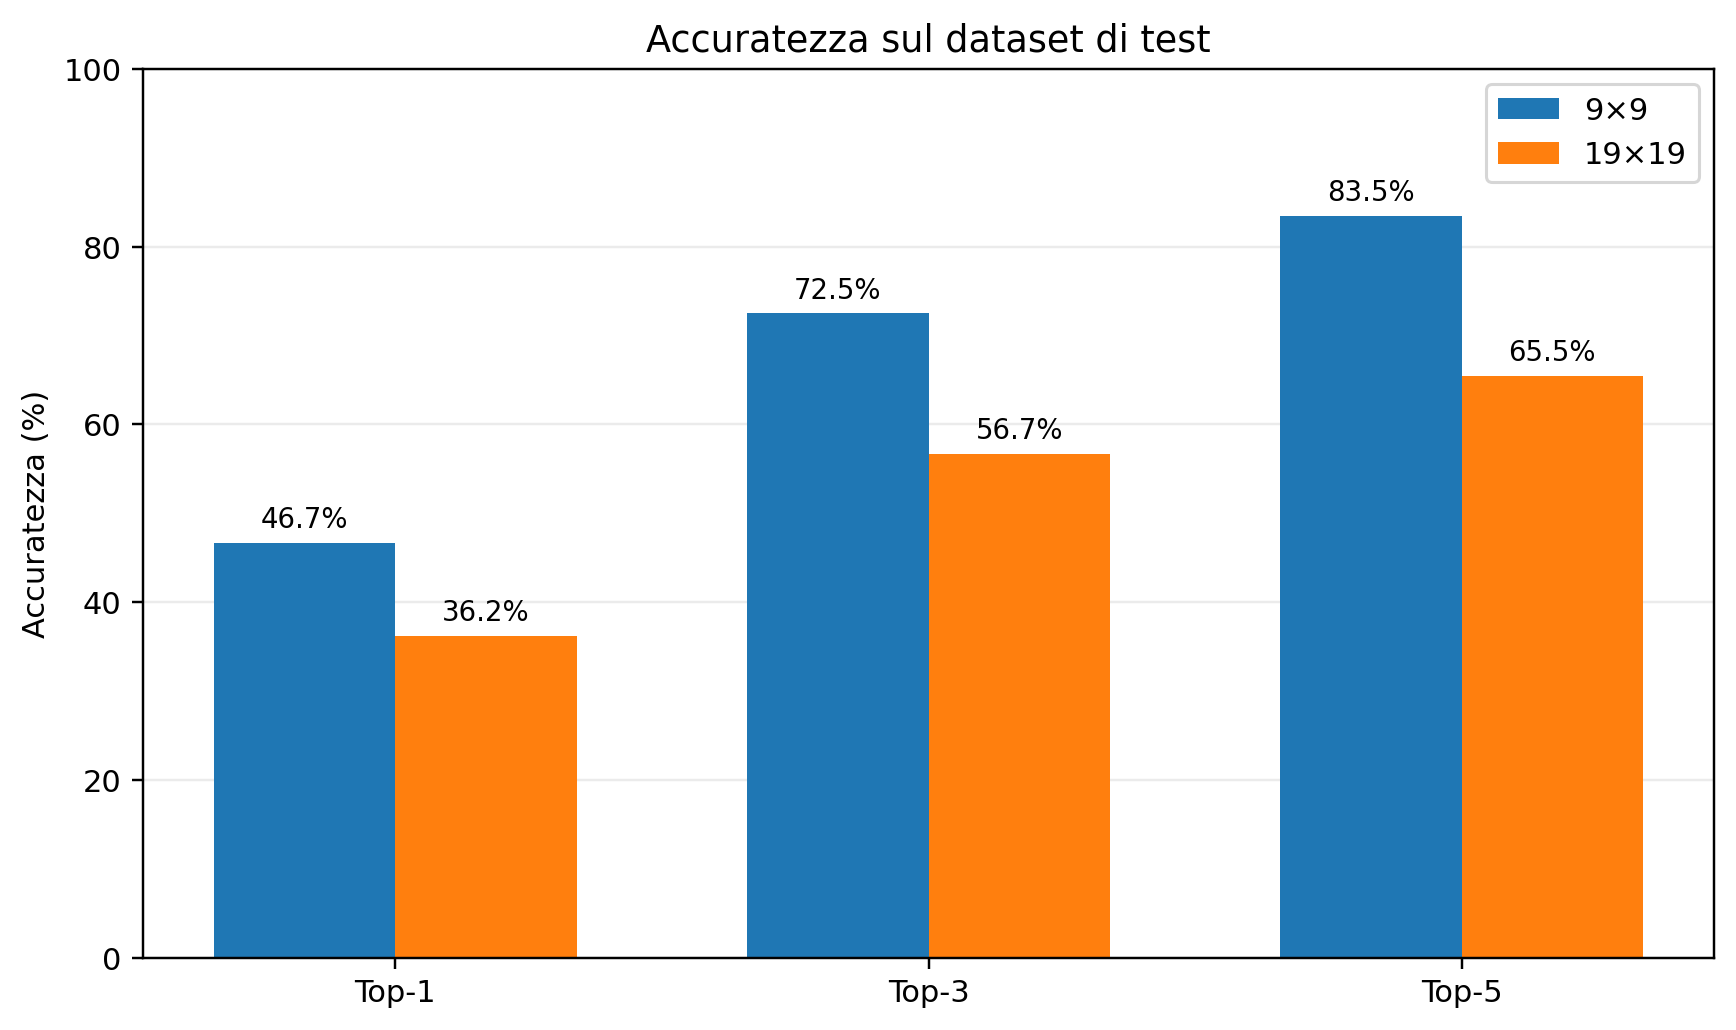
\includegraphics[width=0.85\textwidth]{img/test_accuracy_topk.png}
    \caption{Confronto tra le accuratezze Top-1, Top-3 e Top-5 sui dataset di test.}
    \label{fig:test_topk_accuracy}
\end{figure}

I risultati mostrano prestazioni superiori per la configurazione $9 \times 9$ rispetto a quella $19 \times 19$ su tutte le metriche considerate. Questa differenza deve tuttavia essere interpretata tenendo conto delle diverse dimensioni degli spazi di azione: il modello 9x9 deve scegliere tra 82 azioni, mentre quello 19x19 tra 362.

Inoltre, i due modelli sono stati addestrati su dataset distinti, con un diverso numero di esempi e caratteristiche proprie. Le differenze osservate non possono quindi essere attribuite esclusivamente alla dimensione della scacchiera.

Un ulteriore elemento riguarda la previsione della mossa PASS. Nel dataset di test 9x9 sono presenti 607 esempi PASS, mentre nel dataset 19x19 ne sono presenti 683. Le metriche specifiche di questa classe mostrano risultati differenti: sul 9x9 la precisione è pari al 67,45\% e il recall al 76,11\%; sul 19x19 la precisione raggiunge l'80,68\%, mentre il recall è pari al 55,64\%.

Questi valori evidenziano che la capacità di riconoscere correttamente una mossa di PASS non coincide necessariamente con la capacità di individuare le altre mosse. La distinzione è rilevante, poiché la scelta anticipata di PASS può influenzare significativamente lo svolgimento di una partita.

\subsection{Valutazione contro KataGo}

Per valutare il comportamento degli agenti durante una partita completa, sono stati eseguiti esperimenti contro KataGo, utilizzato come avversario di riferimento.

Per ciascuna dimensione della scacchiera sono state confrontate due configurazioni:
\begin{itemize}
    \item \textbf{Policy}: l'agente seleziona le mosse direttamente dalla distribuzione di probabilità prodotta dalla TRM, dopo aver escluso le azioni illegali.
    \item \textbf{Negamax}: la policy della TRM viene utilizzata per ordinare le mosse candidate, sulle quali viene applicata una ricerca Negamax con potatura alpha-beta.
\end{itemize}

L'obiettivo è verificare se l'introduzione di una ricerca limitata possa migliorare le prestazioni dell'agente rispetto all'utilizzo diretto della policy.

\subsubsection{Configurazione degli esperimenti}

Per ciascuna delle quattro configurazioni sono state giocate 100 partite contro KataGo, alternando il colore assegnato al TRM: 50 partite con il Nero e 50 con il Bianco.

Gli esperimenti sono stati eseguiti utilizzando i seguenti parametri:

\begin{table}[htbp]
    \centering
    \caption{Parametri comuni agli esperimenti contro KataGo.}
    \label{tab:katago_common_config}
    \begin{tabular}{ll}
        \hline
        \textbf{Parametro}         & \textbf{Valore}    \\
        \hline
        Partite per configurazione & 100                \\
        Visite massime KataGo      & 40                 \\
        Profilo HumanSL            & rank\_20k          \\
        Seed                       & 42                 \\
        Komi                       & 7,5                \\
        Penalità sul logit PASS    & 3,5                \\
        Soglia penalità PASS       & 16 pietre occupate \\
        Ricerca Negamax            & Profondità 2       \\
        Candidati Negamax 9x9      & 5                  \\
        Candidati Negamax 19x19    & 3                  \\
        \hline
    \end{tabular}
\end{table}

Per entrambe le dimensioni è stato utilizzato il profilo HumanSL di KataGo denominato \texttt{rank\_20k}. È quindi opportuno precisare che il confronto non è stato effettuato con KataGo alla sua massima forza, ma con una configurazione basata sul profilo umano indicato.

I modelli KataGo utilizzati sono differenti in funzione della dimensione della scacchiera: per il 9x9 è stato impiegato il modello \texttt{kata9x9-b18c384nbt-20231025}, mentre per il 19x19 è stato utilizzato \texttt{kata1-tf3-b11c768-s12382M-d6533M}.

Le partite sono state giocate applicando le regole di scoring ad area, il positional superko e il divieto di suicidio. Il komi è stato impostato a 7,5 punti.

Per confrontare gli agenti sono state considerate principalmente le seguenti metriche:
\begin{itemize}
    \item numero di vittorie, pareggi e sconfitte;
    \item percentuale di vittorie del TRM;
    \item margine medio e mediano delle partite, calcolato dal punto di vista del TRM;
    \item numero medio di mosse per partita;
    \item durata complessiva degli esperimenti e, per Negamax, statistiche della ricerca.
\end{itemize}

Il margine, indicato nel seguito come \textit{gap}, è calcolato sottraendo il punteggio finale di KataGo da quello del TRM. Un valore positivo indica quindi una vittoria o un vantaggio del TRM, mentre un valore negativo indica un vantaggio di KataGo.

\subsubsection{Risultati sul 9x9}

I risultati delle partite sulla scacchiera $9 \times 9$ sono riportati nella Tabella~\ref{tab:katago_9x9}.

\begin{table}[htbp]
    \centering
    \caption{Risultati degli esperimenti contro KataGo sul 9x9.}
    \label{tab:katago_9x9}
    \begin{tabular}{lrr}
        \hline
        \textbf{Metrica} & \textbf{Policy} & \textbf{Negamax} \\
        \hline
        Vittorie TRM     & 26              & 58               \\
        Pareggi          & 0               & 0                \\
        Sconfitte TRM    & 74              & 42               \\
        Win rate         & 26,0\%          & 58,0\%           \\
        Gap medio        & -13,4           & -24,8            \\
        Gap mediano      & -11,5           & +1,5             \\
        Mosse medie      & 64,0            & 98,7             \\
        Durata test      & 2,7 min         & 4,3 min          \\
        \hline
    \end{tabular}
\end{table}

L'introduzione della ricerca Negamax produce un incremento significativo della percentuale di vittorie, che passa dal 26\% al 58\%. La configurazione con ricerca ottiene quindi 32 punti percentuali in più rispetto all'utilizzo diretto della policy.

Si osserva inoltre un aumento del numero medio di mosse per partita, che passa da 64,0 a 98,7. Questo risultato indica che le partite giocate dall'agente con Negamax tendono a proseguire più a lungo.

Il margine medio rimane tuttavia negativo in entrambe le configurazioni. Nel caso di Negamax, la differenza tra margine medio e mediano è particolarmente evidente: il valore mediano è positivo, mentre quello medio è negativo. Ciò suggerisce la presenza di alcune sconfitte con margini particolarmente ampi, capaci di influenzare il valore medio nonostante il maggior numero di vittorie.

\subsubsection{Risultati sul 19x19}

La Tabella~\ref{tab:katago_19x19} riporta i risultati ottenuti sulla scacchiera $19 \times 19$.

\begin{table}[htbp]
    \centering
    \caption{Risultati degli esperimenti contro KataGo sul 19x19.}
    \label{tab:katago_19x19}
    \begin{tabular}{lrr}
        \hline
        \textbf{Metrica} & \textbf{Policy} & \textbf{Negamax} \\
        \hline
        Vittorie TRM     & 48              & 65               \\
        Pareggi          & 0               & 0                \\
        Sconfitte TRM    & 52              & 35               \\
        Win rate         & 48,0\%          & 65,0\%           \\
        Gap medio        & -1,3            & -62,8            \\
        Gap mediano      & -0,5            & +3,5             \\
        Mosse medie      & 216,5           & 393,8            \\
        Durata test      & 17,6 min        & 35,7 min         \\
        \hline
    \end{tabular}
\end{table}

Anche sulla scacchiera $19 \times 19$ la ricerca Negamax determina un incremento della percentuale di vittorie, che passa dal 48\% al 65\%, con un miglioramento di 17 punti percentuali.

Il numero medio di mosse per partita aumenta da 216,5 a 393,8. L'introduzione della ricerca comporta quindi partite mediamente più lunghe e un maggiore costo computazionale.

Anche in questa configurazione si osserva una differenza tra margine medio e mediano. In particolare, il margine medio di Negamax è pari a -62,8 punti, mentre quello mediano è pari a +3,5 punti. Il valore medio risulta pertanto influenzato da alcune sconfitte particolarmente ampie, nonostante il numero complessivo di vittorie sia superiore a quello della policy diretta.

\subsubsection{Confronto tra Policy e Negamax}

La Figura~\ref{fig:katago_winrate} riassume le percentuali di vittoria ottenute nelle quattro configurazioni sperimentali.

\begin{figure}[htbp]
    \centering
    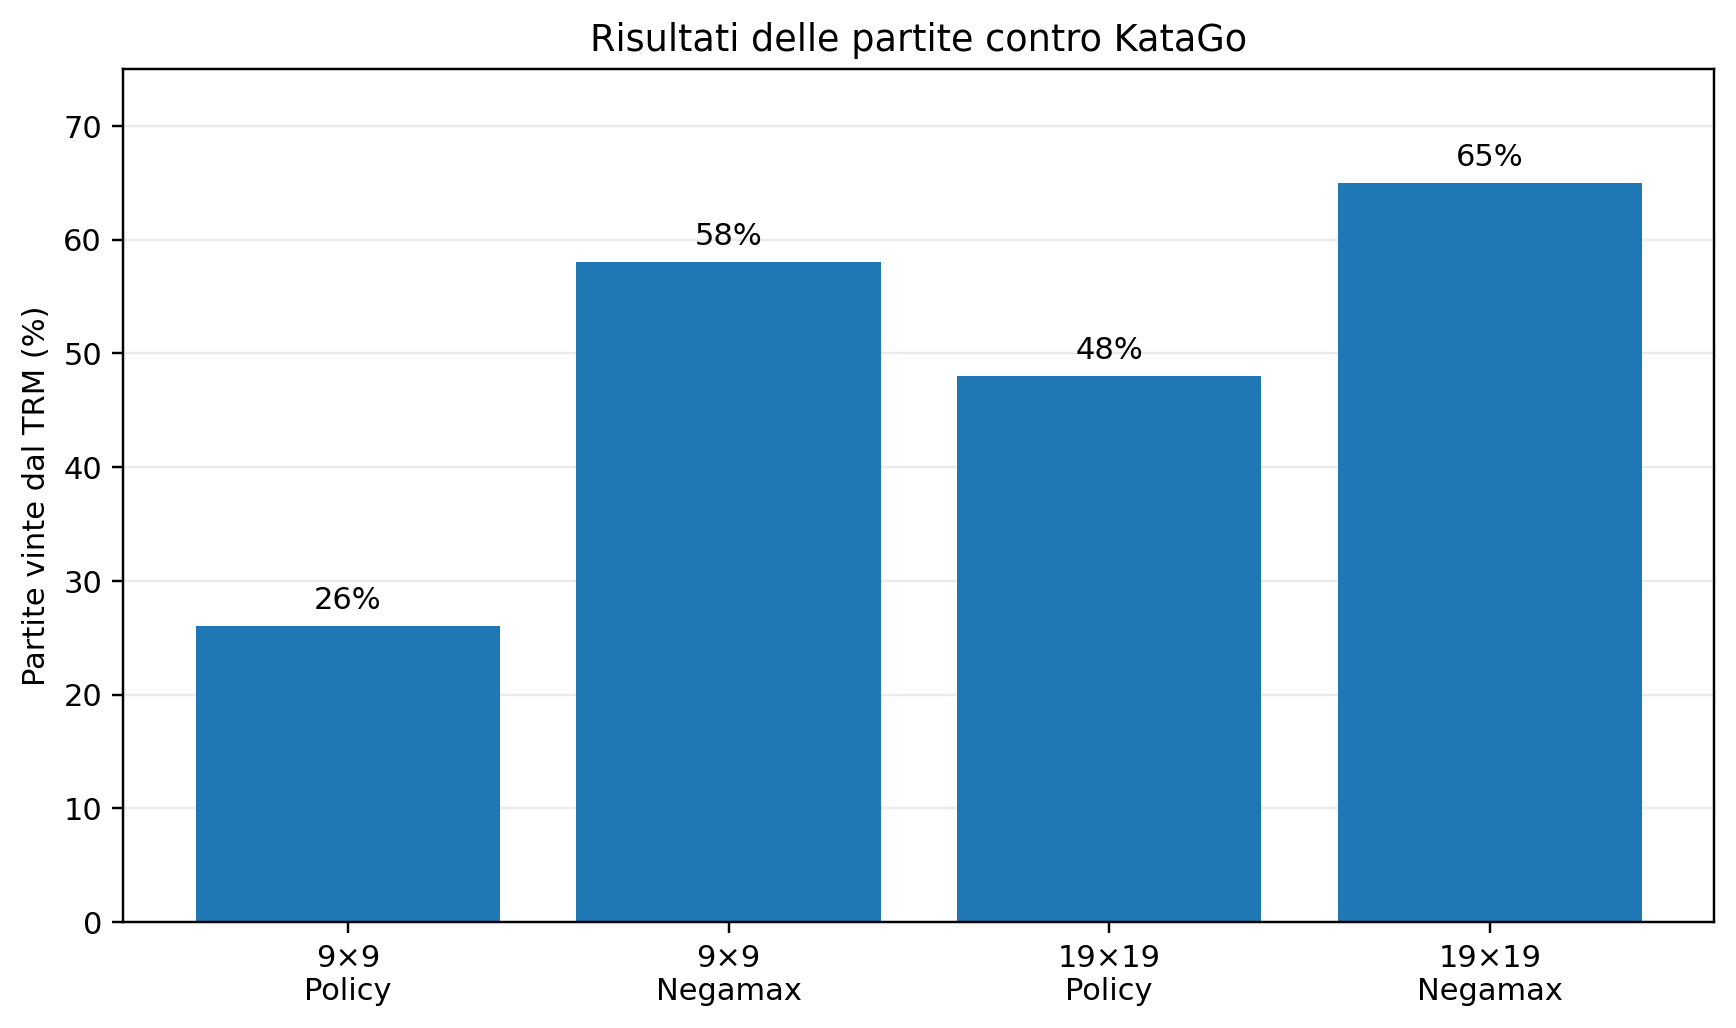
\includegraphics[width=0.85\textwidth]{img/win_rate_katago.png}
    \caption{Percentuale di vittorie del TRM contro KataGo nelle quattro configurazioni sperimentali.}
    \label{fig:katago_winrate}
\end{figure}

In entrambe le dimensioni della scacchiera, l'integrazione della ricerca Negamax migliora la percentuale di vittorie rispetto all'utilizzo diretto della policy.

Il miglioramento è particolarmente evidente nel caso del 9x9, dove la percentuale di vittorie passa dal 26\% al 58\%. Nel caso del 19x19 si osserva invece un incremento dal 48\% al 65\%.

È tuttavia importante considerare che l'aumento delle vittorie non si traduce necessariamente in un miglioramento del margine medio. Come mostrano le tabelle precedenti, alcune sconfitte hanno margini particolarmente elevati e influenzano negativamente la media.

Un ulteriore aspetto riguarda il costo della ricerca. Nel caso del 9x9, il tempo complessivo dedicato alla ricerca Negamax è stato pari a 79,89 secondi, con 123.573 nodi esplorati e 92.770 foglie valutate. Per il 19x19, il tempo complessivo di ricerca è stato pari a 899,38 secondi, con 301.538 nodi esplorati e 218.254 foglie valutate.

Questi valori evidenziano come l'aumento della dimensione della scacchiera comporti un costo computazionale maggiore, anche a parità di profondità di ricerca. La ricerca Negamax permette quindi di migliorare le prestazioni in termini di vittorie, introducendo però un maggiore costo in termini di tempo di esecuzione.

\subsection{Analisi dei risultati e considerazioni}

I risultati ottenuti permettono di formulare alcune considerazioni sull'adattamento della Tiny Recursive Model al gioco del Go.

In primo luogo, la valutazione sui dataset di test mostra che il modello è in grado di individuare la mossa corretta con una certa frequenza, soprattutto considerando un insieme di mosse candidate anziché la sola previsione principale. Le prestazioni risultano differenti tra le due dimensioni della scacchiera, evidenziando la maggiore difficoltà associata allo spazio di azione più ampio del 19x19.

La valutazione contro KataGo evidenzia inoltre un miglioramento della percentuale di vittorie quando la policy viene integrata con una ricerca Negamax. Tale risultato suggerisce che l'utilizzo delle probabilità prodotte dalla TRM per guidare una ricerca limitata può contribuire a migliorare la selezione delle mosse rispetto all'utilizzo diretto della policy.

D'altra parte, i margini medi delle partite mostrano che il numero di vittorie non è sufficiente, da solo, a descrivere completamente le prestazioni dell'agente. In particolare, le differenze tra media e mediana evidenziano la presenza di partite perse con margini molto ampi, che incidono significativamente sul risultato complessivo.

Infine, la ricerca Negamax comporta un aumento del tempo di esecuzione e del numero di operazioni necessarie per selezionare una mossa. Questo aspetto evidenzia il compromesso tra qualità delle decisioni e costo computazionale: una ricerca più articolata può migliorare il comportamento dell'agente, ma richiede risorse aggiuntive.

Nel complesso, gli esperimenti mostrano che la TRM può essere adattata al gioco del Go e utilizzata come componente di una policy per la selezione delle mosse. L'integrazione con una ricerca Negamax limitata rappresenta un ulteriore miglioramento pratico, pur lasciando emergere limiti nella qualità delle decisioni e nella gestione delle situazioni strategicamente più complesse.

\clearpage
% qui secondo me puoi avere due strade diverse: quella "low cost" continuare il training su gpu più potenti in modo da andare ad avere una performance migliore e numero di dati maggiore. oppure quella High cost, ovvero quella di andare a fare Reinforcement learning.

\section{Conclusioni}

\clearpage
\section{Bibliografia}

\begin{thebibliography}{99}

    \bibitem{trm}
    Jolicoeur-Martineau, A.,
    \textit{Less is More: Recursive Reasoning with Tiny Networks},
    2025.

\end{thebibliography}
\clearpage
Ringraziamenti

\end{document}